\chapter{变分推断与确定性近似}
\label{chap:pgm-variational}

第~\ref{chap:pgm-elimination}章的变量消元和第~\ref{chap:pgm-junction-tree}章的团树传播，都是\emph{精确}推断：它们在数学上给出后验边缘和配分函数的准确值。但前面已经反复看到一个瓶颈——计算成本取决于消元过程中出现的最大因子（诱导宽度）。一旦图比较稠密，这个中间团可能包含很多变量，精确推断的时间和存储随团的大小\emph{指数}增长，在现实规模的模型上根本算不动。既然精确答案要不起，一个自然的妥协是\emph{主动放弃一部分精确性、换取可承受的计算量}，但要用可量化的方式做这件事，并能说清近似误差来自哪里。

本章的近似方法沿两条性质不同的路线展开，对应两类不同的查询。第一条针对\textbf{分布查询}（“故障的后验概率是多少”“某统计量的后验期望是多少”）：我们仍然要保留完整的概率与不确定性，做法是\emph{限制后验分布的表达形式}——不在所有可能分布里找后验，而是在一个简单、好算的分布族（如独立乘积分布、高斯）里挑一个“最接近”真实后验的，这就是变分推断。第二条针对\textbf{配置查询}（“所有变量最可能取哪一组值”，即MPE）：此时只要一个最优配置、不需要完整分布，做法是\emph{放宽离散配置的约束}，先把它变成一个更容易解的连续优化问题，再从松弛解恢复出合法配置。两条路线输出不同、误差也要分别衡量。

消元和团树通过中间因子保存变量之间的依赖（第~\ref{chap:pgm-elimination}、\ref{chap:pgm-junction-tree}章）。局部因子虽然很小，中间团却可能包含许多变量，使联合推断的时间和存储成本迅速增长。面对这一瓶颈，我们可以限制后验分布的表达形式，在可计算的分布族中寻找近似；若任务只需要一组最可能的配置，则可以放宽配置约束，先求解较容易的连续优化问题。前一条路线保留概率和不确定性，后一条路线选择离散配置，其误差需要分别衡量。

本章设模型参数已知。对于观测$\bm{x}$和潜变量$\bm{z}$，分布查询以$p(\bm{z}\mid\bm{x})$为目标，计算边缘概率和期望；近似方法可能输出全局分布、局部概率表或高斯近似。配置查询则将证据吸收到因子中，为全部未观测变量选择一组联合最优值，即最可能解释（most probable explanation, MPE）。围绕这两类查询，后文依次讨论近似对象的选择、优化求解与误差诊断。

\section{变分推断的统一视角}

\label{sec:pgm-variational-unified}
\label{sec:pgm-variational-duality}

设备报警后，要判断故障有多大可能，我们需要的是给定报警的状态分布，而不是先选定一种故障状态。推广到一般模型，固定观测$\bm x$和模型参数，用随机向量$\bm Z$表示尚未观测、需要推断的变量。联合模型给出了各个配置的权重$p(\bm x,\bm z)$，后验则要把这些权重归一化：
\[
  \pi(\bm z):=p(\bm z\mid\bm x)
    =\frac{p(\bm x,\bm z)}{p(\bm x)},
  \qquad p(\bm x)=\int p(\bm x,\bm z)\,d\bm z.
\]
本章用积分统一表示连续与离散情形；离散变量的积分改为求和。假设$0<p(\bm x)<\infty$；连续观测下，$p(\bm x)$是观测位置的边缘密度。单个配置的联合权重即使容易评价，累加所有配置仍可能很昂贵。例如，$d$个二元未知变量共有$2^d$种配置；局部分解可减少重复运算，但消元中出现的大团仍可能使计算难以承受。连续变量还可能留下无法解析计算的高维积分。

既然精确后验求不出来，变分法的核心思路是“\emph{用一个好算的分布去近似它}”。但这里立刻冒出两个必须回答的问题：一是用什么标准衡量“近似得像不像”，二是这个标准里仍含着我们算不出的$p(\bm x)$，怎么把它消掉。下面先建立近似分布与候选族的概念，再一步步推出可实际优化的ELBO。如果暂时无法求出$\pi$，可以先构造一个容易查询的分布$q$，用它给同一组未知变量分配概率。对设备模型，固定$A=1$后，$q$仍是$(F,H,S)$上的联合分布，故障概率就用$q(F=1)$近似。若查询的是某个实值统计量$f(\bm Z)$的后验期望，则用$\mathbb E_q f(\bm Z)$近似$\mathbb E_\pi f(\bm Z)$，两者均须存在。这里改变的是计算所用的分布，观测和原模型保持固定。只输出一个配置无法保留这些概率与期望，因此$q$需要描述未知变量的整个分布。

接下来要决定允许使用哪些$q$，以及怎样选出其中较合适的一个。记候选分布族为$\mathcal Q$；例如可用高斯的均值和协方差调整$q$，也可用每个二元变量取$1$的概率规定一个独立乘积分布。若候选写成$q_{\bm\lambda}$，$\bm\lambda\in\Lambda$就是待调整的分布参数，$\Lambda$包含方差为正或概率位于$[0,1]$等约束。调整$\bm\lambda$便是在候选族中选择一个分布，这就是\term{变分推断}（variational inference, VI）将后验计算改写为分布优化的含义\scite{bishop2006,pgm-cmu2017-vi}。

选择$q$需要一个比较准则。反向KL以$q$为积分权重，衡量它与目标后验$\pi$的差异；两者相同时KL为零。因此，我们希望在$\mathcal Q$中减小$D_{\mathrm{KL}}(q\Vert\pi)$。“反向”指参数顺序；本章的$D_{\mathrm{KL}}$和$\operatorname{KL}$表示同一散度。若改用$D_{\mathrm{KL}}(\pi\Vert q)$，期望要在难以查询的真实后验下计算。反向KL把期望放到我们能够控制的$q$下，但它的定义仍含未知的$p(\bm x)$，还需要消去这个计算障碍。

将$\pi(\bm z)=p(\bm x,\bm z)/p(\bm x)$代入KL。因为$\bm x$固定，$\log p(\bm x)$对所有$\bm z$都是同一个常数，又因为$q$的总质量为$1$，便有
\[
  \begin{aligned}
    D_{\mathrm{KL}}(q\Vert\pi)
      &=\mathbb E_q\log\frac{q(\bm Z)}{p(\bm x,\bm Z)}
          +\log p(\bm x)\\
      &=\log p(\bm x)
          -\mathbb E_q\log\frac{p(\bm x,\bm Z)}{q(\bm Z)}.
  \end{aligned}
\]
这一步把目标拆成两项：第一项对所有候选$q$相同，第二项只涉及联合权重和候选分布。比较候选时无需知道第一项的数值，只要增大第二项，就会减小KL。于是将第二项记为证据下界（evidence lower bound, ELBO）：
\begin{equation}
  \begin{aligned}
    \mathcal L(q)
      &:=\mathbb E_q\log\frac{p(\bm x,\bm Z)}{q(\bm Z)},\\
    \log p(\bm{x})
      &=\mathcal L(q)+D_{\mathrm{KL}}(q\Vert\pi).
  \end{aligned}
  \label{eq:pgm-variational-elbo}
\end{equation}
KL非负，所以$\mathcal L(q)\leq\log p(\bm x)$；这解释了“下界”的名称。最大化ELBO同时选择了反向KL意义下更接近后验的候选，而不仅是在估计证据。若采用参数化候选，实际求解的是$\max_{\bm\lambda\in\Lambda}\mathcal L(q_{\bm\lambda})$；所学的是近似后验的参数，原模型参数仍然固定。分布逼近准则、指数族矩表示与最大熵对偶的背景可参考\BookChapterRef{chap:information-theory-and-statistical-geometry}{卷2《数学准备：概率、因果与决策》的“概率分布的分析与优化”章}。下面在本章推断问题中说明所需的关系。

上述有限值分解要求$q\ll\pi$且$D_{\mathrm{KL}}(q\Vert\pi)<\infty$，即$q$不在后验概率为零的集合上放置正质量，并满足相应可积性。这里将ELBO定义为整体对数比的期望；只有两项分别有定义时，才进一步拆成$\mathbb E_q\log p(\bm x,\bm Z)+H(q)$。KL无限时可令ELBO取$-\infty$，但不能在原分解中相加无穷项。消去$p(\bm x)$也不自动保证ELBO容易计算：还需让$q$下的这些期望可以解析求出，或能用采样估计。近似族与计算方法正是围绕这一要求共同选择的\scite{pgm-stanford-cs228-variational}。

从近似族到实际解，还要经过目标选择和数值优化。若$\mathcal Q$无法表示后验，其最优解$q^\star$也会留下近似误差；换用正向KL或矩匹配，则改变了衡量分布差距的准则。对于选定的ELBO，算法得到$\widehat q$后，$\mathcal L(q^\star)-\mathcal L(\widehat q)$衡量尚未消除的优化误差；最优值未取得时，以上确界代替$\mathcal L(q^\star)$。增加迭代主要作用于这一优化差距，近似族的表达限制仍由$\mathcal Q$决定。

反向KL只在$q$分配质量的位置计算对数密度比。若$q$在目标概率为零的区域放置正质量，KL为无穷大；获得有限值要求$q$避开这些区域。这种支持限制称为\term{零强制}（zero forcing），即目标为零迫使近似也为零。正向$\operatorname{KL}(p\Vert q)$的积分权重来自$p$，获得有限值要求$q$覆盖目标的正质量区域，称为\term{零回避}（zero avoiding）。两个名称均描述$q$受到的支持限制\scite{bishop2006}。

支持限制也为模态选择提供了直觉。若正密度目标的两个模态之间存在深谷，单峰$q$同时覆盖两者时，可能在谷底放置较多质量，从而增大反向KL。集中于一个模态可减少这部分代价，因此某些受限近似族会遗漏其他模态。这一倾向取决于目标形状和近似族；足够丰富的混合分布仍可表示多个模态。

相关高斯给出了近似族限制影响方差的可解析例子。设目标$p$是零均值二维高斯，协方差为
\[
  \bm{\Sigma}=
  \begin{pmatrix}1&r\\r&1\end{pmatrix},
  \qquad |r|<1,
\]
并限制$q=\mathcal N(\bm{m},\operatorname{diag}(v_1,v_2))$，其中$v_1,v_2>0$。这个限制允许调整两个边缘的均值和方差，却不能用协方差表达目标中的相关性。记精度矩阵为
\[
  \bm\Lambda=\bm\Sigma^{-1}
    =\frac{1}{1-r^2}
      \begin{pmatrix}1&-r\\-r&1\end{pmatrix}.
\]
将两个高斯的对数密度代入反向KL，并使用$\mathbb E_q\bm Z=\bm m$及$\operatorname{Cov}_q(\bm Z)=\operatorname{diag}(v_1,v_2)$，得到
\[
  \operatorname{KL}(q\Vert p)
    =\frac12\left\{
       \bm m^\top\bm\Lambda\bm m
       +\sum_i\bm\Lambda_{i,i}v_i-2
       +\log\det\bm\Sigma-\sum_i\log v_i\right\}.
\]
其中$-2+\log\det\bm\Sigma$只依赖固定目标。舍去这类与候选参数无关的常数后，需要最小化的有关项为
\[
  \frac12\left\{\bm{m}^{\top}\bm{\Lambda}\bm{m}
     +\sum_i\bm{\Lambda}_{i,i}v_i-\sum_i\log v_i\right\}.
\]
均值项的梯度为$\bm\Lambda\bm m$；$\bm\Lambda$正定，因此这一项在$\bm m=\bm0$处取得唯一最小值。每个方差项的导数为$\tfrac12(\bm\Lambda_{i,i}-1/v_i)$，二阶导数为$1/(2v_i^2)>0$。令一阶导数为零，便得到唯一最优方差
\[
  v_i=\frac{1}{\bm\Lambda_{i,i}}=1-r^2.
\]

取$r=0.8$时，目标的两个边缘方差均为$1$，最优独立近似却均为$0.36$。二维高斯中，给定另一坐标后的条件方差为$1-r\cdot1^{-1}\cdot r=1-r^2$，恰好等于这里的独立近似方差。它比目标的边缘方差更小。

换成正向$\operatorname{KL}(p\Vert q)$时，积分权重来自目标$p$。因为目标每个坐标的均值为$0$、二阶矩为$1$，依赖候选参数的部分变成
\[
  \frac12\sum_i\left\{\log v_i+\frac{1+m_i^2}{v_i}\right\}.
\]
对固定$v_i$，$m_i^2/v_i$在$m_i=0$处最小；代回后，对$v_i$求导得到$\tfrac12(1/v_i-1/v_i^2)$，其符号在$v_i=1$两侧由负变正。于是正向KL的最优解匹配边缘矩，得到$\bm m=\bm0$和$v_i=1$。因此，在这一相关高斯和独立高斯近似族的设定下，反向KL最优解低估边缘方差；结论的范围由这两个分布族共同限定。

优化整个$q$后，可以由它计算各个节点或因子的边缘概率。不过，许多查询只需这些小表，我们也希望直接以局部概率表作为优化变量。两种表示怎样连接？对离散节点，事件$Z_i=k$的概率等于指示函数$\mathbb I\{Z_i=k\}$的期望；一组变量的联合配置概率同样可以这样表示。将所需指示函数收集为统计量向量$\bm T$，其期望就收集了局部概率表。下面先用指数族说明模型得分怎样作用于这些期望，再检查哪些局部表能够来自同一个联合分布。记自然参数为$\bm\theta$，它在此表示固定模型的得分系数：
\begin{equation}
  \begin{aligned}
    p_{\bm{\theta}}(\bm{z})
      &=h(\bm{z})\exp\{\langle\bm{\theta},\bm{T}(\bm{z})\rangle
                      -A(\bm{\theta})\},\\
    A(\bm{\theta})
      &=\log\int h(\bm{z})
          e^{\langle\bm{\theta},\bm{T}(\bm{z})\rangle}\,d\bm{z}.
  \end{aligned}
  \label{eq:pgm-variational-exponential-family}
\end{equation}
$h$为不依赖参数的基准项，$A$为对数配分函数。

要由模型参数读出这些局部概率，需要计算$\bm T$的期望。自然参数位于$A<\infty$的开域内且可交换微分与积分时，对归一化积分求导，再除以该积分，得到
\[
  \frac{\partial A}{\partial\theta_j}
    =\frac{\int T_j(\bm z)h(\bm z)
                  e^{\langle\bm\theta,\bm T(\bm z)\rangle}\,d\bm z}
           {\int h(\bm z)e^{\langle\bm\theta,\bm T(\bm z)\rangle}\,d\bm z}
    =\mathbb E_{\bm\theta}T_j(\bm Z).
\]
再次对$\theta_k$求导时，分子的导数产生$\mathbb E(T_jT_k)$，分母的导数产生$\mathbb E T_j\mathbb E T_k$。两项相减就是协方差，因此
\begin{equation}
  \nabla A(\bm{\theta})=\mathbb E_{\bm{\theta}}\bm{T}(\bm{Z})
      =:\bm{\mu},\qquad
  \nabla^2 A(\bm{\theta})
      =\operatorname{Cov}_{\bm{\theta}}[\bm{T}(\bm{Z})].
  \label{eq:pgm-variational-moments}
\end{equation}
$\bm{\mu}$称为\term{均值参数}（mean parameter），直接记录期望统计量。

均值参数能否反过来确定自然参数，取决于统计量是否重复记录了同一信息。例如，若保留某节点全部状态的指示函数，就恒有$\sum_k\mathbb I\{Z_i=k\}=1$。沿这些自然参数同时加上同一个常数，只会把每个配置的未归一化权重乘以同一常数；归一化后的分布和均值参数都不改变。这就是一条仿射冗余：某个非零系数向量$\bm a$使$\langle\bm a,\bm T(\bm z)\rangle$在共同支持上几乎处处为常数。

式~\eqref{eq:pgm-variational-moments}还说明了冗余为何产生Hessian零方向，因为
\[
  \bm a^\top\nabla^2A(\bm\theta)\bm a
    =\operatorname{Var}_{\bm\theta}
          [\langle\bm a,\bm T(\bm Z)\rangle]=0.
\]
删去这些关系中可由其余统计量和常数表示的冗余分量，保留足以表示同一分布族的一组统计量，便得到这里所需的最小表示。在共同支持上密度为正、协方差存在且上述求导有效时，最小表示中的每个非零方向都有正方差，Hessian因而正定。自然参数取合法开域中的有限值时，逆函数定理便给出$\bm\theta\mapsto\bm\mu$的局部一一对应。

这里的内部条件同时限定参数和待匹配的矩。我们要求使用合法开域中的有限自然参数，并要求目标矩属于这些参数能够实现的内部均值域；仅仅写下一组数值，并不能保证它们是该分布族的矩。下文的有限离散模型在删除仿射冗余后，其内部均值域就是可实现集合的相对内部，即在该集合实际所在的仿射空间内取内部。边界矩可能仍能由某个分布实现，却只能由指数族中的参数极限逼近，不能套用上述局部可逆性。

将局部表直接当作优化变量时，逐表归一化还不够。例如，两个表若都包含同一节点，却给该节点不同的边缘概率，就不可能来自同一个联合分布。我们因此需要描述所有可由联合分布实现的统计量期望。以下对偶与多面体陈述先限定为有限离散状态、$h=1$。以$V=\{1,\ldots,d\}$记节点集，$Z_i$的有限非空状态集为$\mathcal X_i$，节点集$A\subseteq V$上的配置集为$\mathcal X_A=\prod_{i\in A}\mathcal X_i$，全部联合配置组成$D=\mathcal X_V$。定义\term{边缘多面体}（marginal polytope）
\begin{equation}
  \mathcal M
    =\left\{\mathbb E_q\bm{T}(\bm{Z}):q\text{为全局分布}\right\}
    =\operatorname{conv}\{\bm{T}(\bm{z}):\bm{z}\in D\},
  \label{eq:pgm-variational-marginal-polytope}
\end{equation}
其中$\operatorname{conv}$表示凸包。这个等号来自$\mathbb E_q\bm T=\sum_{\bm z\in D}q(\bm z)\bm T(\bm z)$：概率$q(\bm z)$是非负且总和为$1$的凸组合系数；反过来，每一组这样的系数都定义一个全局分布。当$\bm{T}$由节点和因子配置的指示函数组成时，$\bm{\mu}$就是相应边缘概率。$\mathcal M$要求这些局部表格能够同时来自某个全局分布，而不只是每张表各自归一化。

有了可实现的均值参数，还要说明为什么只看期望得分不足以计算配分函数。在当前有限离散、$h=1$的设定下，对任意全局分布$q$，将$p_{\bm\theta}$代入KL可得
\[
  \operatorname{KL}(q\Vert p_{\bm\theta})
    =A(\bm\theta)-\langle\bm\theta,\mathbb E_q\bm T\rangle-H(q).
\]
KL非负，且$q=p_{\bm\theta}$时取零，所以在所有$q$中最大化期望得分加熵，恰好得到$A(\bm\theta)$。这里的熵保留了不同配置共同贡献的概率质量；只取一个配置的得分，还没有累计这些贡献。

现在按$\mathbb E_q\bm T=\bm\mu$将候选分布分组。同一组中，$\langle\bm\theta,\bm\mu\rangle$完全相同，差别只在熵，因此先选这一组中熵最大的分布，再比较不同的$\bm\mu$。对$\bm\mu\in\mathcal M$，令$H^\star(\bm\mu)=\max_{q:\mathbb E_q\bm T=\bm\mu}H(q)$，即满足这些统计量约束的分布所能达到的最大熵。有限状态下，约束分布集合非空且紧，熵连续，所以这一最大值存在。这样便得到
\begin{equation}
  A(\bm\theta)=\max_{\bm\mu\in\mathcal M}
    \{\langle\bm\theta,\bm\mu\rangle+H^\star(\bm\mu)\}.
  \label{eq:pgm-variational-gibbs}
\end{equation}
这一优化包含$\mathcal M$的边界，不要求每个候选均值都由有限自然参数实现。例如，对单个伯努利变量取$T(z)=z$，确定性分布$q(Z=1)=1$给出边界均值$\mu=1$和熵$0$；有限自然参数产生的概率$e^\theta/(1+e^\theta)$始终小于$1$，只有$\theta\to+\infty$才到达该边界极限。边界仍是合法候选，因为这里的优化域由所有全局分布确定。

还可以反过来，固定$\bm\mu$，考察线性项减去对数配分函数所得的差值，并在自然参数上取上确界：
\[
  A^*(\bm\mu)
    :=\sup_{\bm\theta}
          \{\langle\bm\theta,\bm\mu\rangle-A(\bm\theta)\}.
\]
这个函数称为$A$的凸共轭。式~\eqref{eq:pgm-variational-gibbs}说明，对可实现的$\bm\mu$，花括号中的量始终不超过$-H^\star(\bm\mu)$。有限离散模型的熵对偶进一步给出
\[
  A^*(\bm\mu)=
    \begin{cases}
      -H^\star(\bm\mu),&\bm\mu\in\mathcal M,\\
      +\infty,&\bm\mu\notin\mathcal M.
    \end{cases}
\]
内部均值处，可以用实现最大熵分布的自然参数达到等号；边界处需要允许上确界由参数极限实现。这一关系的用途是把分布优化改写为均值坐标上的优化：可实现性由$\mathcal M$承担，分布在相同矩约束下还能保留多少不确定性由$H^\star$承担。该表示因此将图推断的困难集中到可行域$\mathcal M$和最大熵$H^\star$上。

凸共轭中的负熵对应给定统计量约束下的最大熵。少量边缘统计量通常容许多个全局分布；这些分布具有相同的得分期望，熵却可能不同，故它们各自的熵未必等于$H^\star$。基准项为一般$h$时，熵项相应变为$H(q)+\mathbb E_q\log h$。连续变量还涉及可积性、闭性和对偶成立条件，其均值可实现集合通常也超出有限多面体的范围。指数族与变分对偶的系统论述见Wainwright和Jordan\scite{pgm-wainwright2008}。

式~\eqref{eq:pgm-variational-gibbs}中的计算困难有两个来源：描述$\mathcal M$可能需要大量全局一致性约束，计算$H^\star$可能需要恢复联合分布。平均场限制全局分布族并计算真实熵，从而得到对数配分函数下界；局部自由能方法则同时近似可行集合和熵，界的方向取决于具体构造。对于配置优化，目标中没有熵，扩大可行集合直接给出最大得分上界。

同一坐标也能表示MPE。令$S(\bm z)=\langle\bm{\theta},\bm T(\bm z)\rangle$为吸收证据后的有限离散得分，$D$为全部未观测变量的完整配置集合，则
\begin{equation}
  \max_{\bm z\in D}S(\bm z)
    =\max_{\bm{\mu}\in\mathcal M}
       \langle\bm{\theta},\bm{\mu}\rangle.
  \label{eq:pgm-variational-mpe}
\end{equation}
这一等号可直接由凸组合看出：任意$\bm\mu\in\mathcal M$都给出$\langle\bm\theta,\bm\mu\rangle=\sum_{\bm z}q(\bm z)S(\bm z)$，加权平均不超过最大配置得分；把$q$集中在某个最大得分配置上，又能取到这个最大值。右侧没有熵项，因为答案只需保留一个最大得分配置，而无须累计其他配置的概率质量。对数配分函数查询若替换$\mathcal M$或$H^\star$，误差落在分布、边缘或归一化常数上；MPE若扩大$\mathcal M$，则得到连续松弛及最大得分上界，还必须从松弛解恢复合法配置。这正是两条主线共享几何表示而输出、保证和诊断不同的原因。

共同的统计量坐标便于比较近似方法所改变的对象。拉普拉斯近似用众数附近的二阶展开替代对数密度，EP通过临时放回真实因子后的分布匹配矩，两者将在第~\ref{sec:pgm-variational-laplace-ep}节说明。LP从无熵的式~\eqref{eq:pgm-variational-mpe}出发，放宽配置的一致性约束（第~\ref{sec:pgm-variational-lp}节）。这三种机制分别改变密度形状、局部矩和可行集合，对应不同的误差与诊断。

\begin{example}[三角图的精确基准]
  \label{ex:pgm-variational-triangle}
  以下人工构造的二元模型贯穿本章。三个变量$Z_i\in\{0,1\}$组成三角图，每条边奖励端点取不同值：
  \begin{equation}
    p_\beta(\bm{z})=\frac{\exp S_\beta(\bm{z})}{Z_\beta},
    \qquad
    S_\beta(\bm{z})
      =\beta\sum_{(i,j)\in E}\mathbb I[z_i\ne z_j],
    \quad \beta=\log2.
    \label{eq:pgm-variational-triangle}
  \end{equation}
  两个全相同配置的得分为$0$，其余六个配置恰有两条不相等边，得分为$2\beta$。将八个配置的权重相加，得到
  \[
    Z_\beta=2+6e^{2\beta}=26.
  \]
  接着固定边$(1,2)$的状态，只对$Z_3$求和。若$(Z_1,Z_2)=(0,0)$，$Z_3=0$和$Z_3=1$的权重分别为$1$和$e^{2\beta}=4$，所以这一边状态的边缘概率为$5/26$。若$(Z_1,Z_2)=(0,1)$，无论$Z_3$取何值，都恰有两条异值边；两个权重均为$4$，相加得到$8/26=4/13$。同时翻转全部变量不会改变得分，因此$(1,1)$与$(0,0)$同概率，$(1,0)$与$(0,1)$同概率。每条边的概率表于是为
  \[
    p_\beta(Z_i,Z_j)=
      \begin{pmatrix}5/26&4/13\\4/13&5/26\end{pmatrix},
      \qquad (i,j)\in E,
  \]
  其中行、列依次按状态$0,1$排列。由表格沿任一行或列求和，得到$p_\beta(Z_i=1)=5/26+4/13=1/2$；将两个非对角项相加，得到$p_\beta(Z_i\ne Z_j)=8/13$。每条边的两个同值状态$(0,0)$与$(1,1)$因而各有概率$5/26$，两个异值状态$(0,1)$与$(1,0)$各有概率$4/13$。节点边缘都是均匀的，但节点并不独立；三个二元变量也不可能在每条边上都取不同值：若$Z_1\ne Z_2$且$Z_2\ne Z_3$，二元性就迫使$Z_1=Z_3$，与第三条边也要求异值矛盾。
\end{example}

图~\ref{fig:pgm-variational-triangle}把同一模型的三种描述并列起来。中间面板使用本例的均匀平均场解，即每个$q_i(Z_i=1)=1/2$；后文将求出这个解并检查它的最优性。在这个特定乘积分布中，一条边取不同值的概率是$1/2$。一般乘积分布的这一概率还会随两个节点的边缘改变，不能仅由完全因子化就断定为$1/2$。完全因子化近似丢失节点相关性，局部一致表则可能提出无法共同实现的边缘。后文用这个模型分别检查分布近似和配置松弛的误差。
\begin{figure}[htbp]
  \centering
  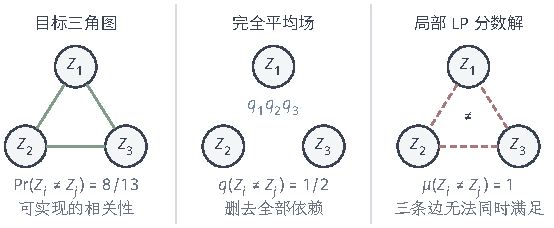
\includegraphics[width=92.445mm]{figures/06-probabilistic-graphical-models/02-inference/tikz/pgm-variational-triangle/figure.pdf}
  \caption{三角图、完全因子化分布和局部一致的边缘表。中间为本例均匀平均场解$q_i(Z_i=1)=1/2$，其边异值概率为$1/2$。右侧让每条边都以概率$1$取不同值，节点边缘仍都是$(1/2,1/2)$；它满足局部一致性，却不可能由任何全局二元分布实现。}
  \label{fig:pgm-variational-triangle}
\end{figure}

\section{近似后验分布与边缘概率}

\label{sec:pgm-variational-posterior}

后验分布或边缘概率难以精确求出时，需要回答三个问题：怎样构造可计算的近似，怎样求出这个近似，以及它能否可靠地回答所需的查询。下面依次讨论后验分布与边缘概率的近似、近似的计算和近似的可靠性。

\subsection{后验分布与边缘概率的近似}
\label{sec:pgm-variational-laplace-ep}

限制全局分布、放宽局部边缘的一致性、匹配分布矩和近似局部曲率，改变的是不同的概率对象与近似准则。各方法的更新公式在构造中一并给出；随后再讨论如何组织这些计算。

\subsubsection{基于因子化分布的近似}

\label{sec:pgm-variational-mean-field}
\label{sec:pgm-variational-mean-field-structured}
\label{sec:pgm-variational-coordinate}

完整联合概率表要记录每一种变量组合，$d$个二元变量就需要$2^d-1$个自由概率，这正是精确推断扛不住的原因。最简单的“砍参数”办法是假设推断时各变量\emph{相互独立}：只保存每个变量自己的边缘分布（$d$个二元变量只需$d$个数），再把它们相乘当作联合分布。这样做当然丢掉了变量之间的相关性——但原模型里的耦合并没有消失，它会在逐个更新某个变量时、通过“其他变量的期望”重新进入计算。\term{平均场近似}（mean-field approximation）采用
\[
  q(\bm{z})=\prod_{i=1}^{d}q_i(z_i).
\]
在$q$中，各变量相互独立，条件分布因而不随其他变量的取值改变。原模型的耦合仍通过期望进入坐标更新，因子化简化的是近似分布的表达。

因子化之后，仍要选择各个$q_i$，使整个乘积分布的ELBO尽量大。可以先保持其他因子不变，只调整一个$q_i$，再依次轮换；这相当于把一次联合优化拆成多次单因子优化。这里固定的是其他变量的分布，而非其他变量的某个取值。记$q_{-i}=\prod_{j\ne i}q_j$，并定义$a_i(z_i)=\mathbb E_{q_{-i}}\log p(\bm{x},z_i,\bm{Z}_{-i})$。ELBO中依赖$q_i$的部分为
\[
  \int q_i(z_i)a_i(z_i)\,dz_i-\int q_i(z_i)\log q_i(z_i)\,dz_i.
\]
假设$C_i=\int e^{a_i(z_i)}dz_i$有限且为正，令$q_i^\star=e^{a_i}/C_i$，上述表达式就等于$\log C_i-\operatorname{KL}(q_i\Vert q_i^\star)$。KL在两分布相同时取唯一最小值，因此得到最优坐标更新：
\begin{equation}
  q_i^\star(z_i)
    \propto\exp\left\{\mathbb E_{q_{-i}}
      [\log p(\bm{x},z_i,\bm{Z}_{-i})]\right\}.
  \label{eq:pgm-variational-coordinate}
\end{equation}
期望只对其他变量计算，$z_i$在这一步是保留的自变量。更新使用的是对数联合分布的期望，再取指数；一般不等于$\mathbb E_{q_{-i}}p(z_i\mid\bm{x},\bm{Z}_{-i})$，也不等于把其他变量一律替换为其均值。

若原模型按因子分解，所有不含$z_i$的项都是归一化时可去掉的常数。平均场因此仍能局部更新。对例~\ref{ex:pgm-variational-triangle}，现在直接使用未归一化得分$S_\beta$，定义对数配分函数下界
\begin{equation}
  \begin{aligned}
    \mathcal L_Z(q)&=\mathbb E_qS_\beta(\bm Z)+H(q),\\
    \operatorname{KL}(q\Vert p_\beta)
      &=\log Z_\beta-\mathcal L_Z(q).
  \end{aligned}
  \label{eq:pgm-variational-partition-lower-bound}
\end{equation}
因此$\mathcal L_Z(q)\leq\log Z_\beta$。若使用已归一化的$p_\beta$计算$\mathbb E_q\log p_\beta+H(q)$，结果则是$\mathcal L_Z(q)-\log Z_\beta\leq0$，两者相差一个与$q$无关的常数。

令$m_i=q_i(Z_i=1)$。在乘积分布中，两节点取不同值分为互斥的两种情况：$Z_i=1,Z_j=0$与$Z_i=0,Z_j=1$。由独立性，它们的概率之和为
\[
  q(Z_i\ne Z_j)
    =m_i(1-m_j)+(1-m_i)m_j
    =m_i+m_j-2m_im_j.
\]
每条边的期望得分就是这个概率乘以$\beta$。乘积分布的熵等于各伯努利熵之和；记$h_{\mathrm B}(m)=-m\log m-(1-m)\log(1-m)$，并按连续延拓约定$h_{\mathrm B}(0)=h_{\mathrm B}(1)=0$。将得分与熵合并，并记$\mathcal L_{\mathrm{MF}}(\bm m)=\mathcal L_Z(\prod_iq_i)$，便得到下面第一行的目标；第二行是由它求出的坐标更新：
\begin{equation}
  \begin{aligned}
    \mathcal L_{\mathrm{MF}}(\bm m)
      &=\beta\sum_{(i,j)\in E}
           (m_i+m_j-2m_im_j)+\sum_i h_{\mathrm B}(m_i),\\
    m_i^{\mathrm{new}}
      &=\sigma\left(\beta\sum_{j\in N(i)}(1-2m_j)\right),
  \end{aligned}
  \label{eq:pgm-variational-triangle-mf}
\end{equation}
其中$\sigma(u)=1/(1+e^{-u})$，$N(i)$是相邻节点集合。为了看清第二行的来源，固定其他$m_j$，对第一行关于$m_i$求导：
\[
  \frac{\partial\mathcal L_{\mathrm{MF}}}{\partial m_i}
    =\beta\sum_{j\in N(i)}(1-2m_j)
       +\log\frac{1-m_i}{m_i}.
\]
令该导数为零并移项，就得到$\log\{m_i/(1-m_i)\}=\beta\sum_{j\in N(i)}(1-2m_j)$。解出$m_i$，正是式~\eqref{eq:pgm-variational-triangle-mf}中的坐标更新。若两个邻居的$m_j$均为$1/4$，两项$(1-2m_j)$之和为$1$，新$m_i=\sigma(\log2)=2/3$；邻居偏好$0$，当前变量便更偏好$1$。更新后的$m_i$仍表示伯努利分布中的概率，保留当前变量的不确定性。

均匀初始化给出固定点$m_i=1/2$，因为每个$(1-2m_j)$都为零，更新仍返回$\sigma(0)=1/2$。此时三条边各以概率$1/2$取不同值，期望得分为$3\beta/2$；三个节点各贡献熵$\log2$。因此其对数配分函数下界为$\mathcal L_{\mathrm{MF}}=(9/2)\log2\approx3.119162$，低于$\log26\approx3.258097$。

这一例中，均匀固定点还是平均场的唯一全局最优点。先在$0<m_i<1$内计算目标Hessian：对角元为$-1/[m_i(1-m_i)]\leq-4$，相邻两节点对应的非对角元为$-2\beta$。三角图中每行恰有两个这样的非对角元，所以对任意向量$\bm u$，利用$2|u_i u_j|\leq u_i^2+u_j^2$可得
\[
  \bm u^\top\nabla^2\mathcal L_{\mathrm{MF}}\bm u
    \leq(-4+4\beta)\lVert\bm u\rVert_2^2.
\]
这里$\beta=\log2<1$，故最大特征值不超过$-4+4\beta<0$，目标在内部严格凹。

还须排除最大值出现在边界的可能。固定其他节点时，得分关于$m_i$是斜率有限的线性函数，而伯努利熵的导数$\log\{(1-m_i)/m_i\}$在$m_i\to0$时趋于$+\infty$，在$m_i\to1$时趋于$-\infty$。因此从任一端点向内部移动足够小的距离，都能增加目标。目标在闭立方体$[0,1]^3$上连续，最大值存在；边界不能取最大值，内部严格凹且均匀点的梯度为零，所以均匀点就是唯一全局最大点。

即使如此，该最优乘积分布仍给出$q(Z_i\ne Z_j)=1/2$，低于真实的$8/13$。这一差距来自独立近似族的表达限制，即使达到其全局最优仍会保留。

\par\noindent\begin{minipage}{\linewidth}
\begin{algorithm}[循环坐标平均场]
  \label{alg:pgm-variational-cavi}
  \begin{algorithmic}[1]
    \Require 联合分布、因子化近似族、有限ELBO的初值$q$、可归一化的坐标更新、容差$\varepsilon>0$、最大轮数$T_{\max}\in\mathbb N_{>0}$
    \Ensure 近似分布$q$及其ELBO
    \State 计算当前ELBO，令轮数$t\gets0$
    \Repeat
      \State 保存本轮开始时的ELBO
      \For{$i=1,\ldots,d$}
        \State 用其他因子的最新值计算式~\eqref{eq:pgm-variational-coordinate}
        \State 归一化并替换$q_i$
      \EndFor
      \State 重新计算ELBO及本轮增量，令$t\gets t+1$
    \Until{增量不超过$\varepsilon$，或$t\geq T_{\max}$}
  \end{algorithmic}
\end{algorithm}
\end{minipage}\par

算法~\ref{alg:pgm-variational-cavi}将一遍完整坐标扫描记为一轮，以$T_{\max}$给出计算预算。停止时输出的是当前近似分布；达到预算本身不表示目标增量已经小于容差。算法依次使用其他因子的最新值，精确最大化每个坐标。因此，把同一更新持续执行时，ELBO单调不减，又以对数证据为上界，目标值序列收敛。参数序列收敛和一般模型的全局最优还需要其他条件。同时使用旧值并行更新所有坐标时，更新之间相互影响，上述逐坐标单调性论证不适用。

完全独立的平均场有时砍得太狠——比如一条隐藏状态链上相邻状态高度相关，硬把它们当独立会丢掉最关键的轨迹协调关系。一个折中是\emph{有选择地}在近似分布$q$里保留一部分依赖：把变量分成若干块，块与块之间独立，块内部仍做（可能精确的）联合推断。这样表达力比完全平均场强，代价是每块的更新更贵。单变量因子化会拆开后验中的重要依赖。例如，相邻隐状态高度相关时，独立边缘无法表达一条轨迹上状态选择的协调关系。\term{结构化变分推断}（structured variational inference）在$q$中保留选定的依赖，通过块内推断计算相关状态的联合概率。表达能力由此增强，局部更新的成本也随之增加。
\label{sec:pgm-variational-structured}

一种直接选择是把节点划分成互不相交的块$B_1,\ldots,B_K$，并让不同块独立，即
\[
  q(\bm z)=\prod_k q_k(\bm z_{B_k}).
\]
与单变量推导相同，固定其余块后，当前块的最优分布满足
\begin{equation}
  q_k^\star(\bm z_{B_k})
     \propto\exp\left\{
       \mathbb E_{q_{-B_k}}\log p(\bm x,\bm z_{B_k},\bm Z_{-B_k})
     \right\}.
  \label{eq:pgm-variational-block}
\end{equation}
块内部原有相互作用被保留，跨块作用转成期望势。链与小树都可以沿用第~\ref{sec:pgm-junction-tree-sum-product}节的和积消息；在链上向两个方向传递消息，就是后文时序模型使用的前向--后向计算。若是稠密大块，更新仍会遇到指数级枚举。因此，块大小只是粗略指标，块内树宽和因子的代数结构才决定计算代价。

回到三角图，取$q(z_1,z_2)q(z_3)$并令$q(z_3=1)=1/2$。固定任一$z_1,z_2$时，均匀的$Z_3$与$z_1$取不同值的概率是$1/2$，与$z_2$取不同值的概率也是$1/2$。因此对$Z_3$求期望后，两条跨块边的得分总和恒为$\beta$，不会改变块$(Z_1,Z_2)$内各配置的相对权重。块内得分仍为$\beta\mathbb I[z_1\ne z_2]$，将四个配置的权重归一化便得
\[
  q(z_1,z_2)=
    \frac{e^{\beta\mathbb I[z_1\ne z_2]}}{2+2e^\beta}.
\]
记$C=2+2e^\beta$。两个异值配置的总权重是$2e^\beta$，所以当$\beta=\log2$时，块内不同值的概率为$2e^\beta/C=2/3$。同时翻转$Z_1,Z_2$不会改变块分布，因此两个节点的边缘仍均为$(1/2,1/2)$。反过来更新$q(z_3)$时，这两个均匀边缘使两条跨块边对任一固定$z_3$的期望得分都为$\beta/2$；总得分不随$z_3$改变，更新仍返回均匀分布。这样就验证了两个方向的块坐标更新都不再改变当前解，故它是块坐标固定点。两条跨块边的不同值概率仍为$1/2$。

为了计算这一近似给出的下界，对块分布的对数取期望，得到
\[
  H(q_{1,2})=\log C-\beta q(Z_1\ne Z_2).
\]
块内期望得分为$\beta q(Z_1\ne Z_2)$，恰好与上式第二项相消。再加上跨块期望得分$\beta$和$q_3$的熵$\log2$，便有$\mathcal L_Z=\log(2+2e^\beta)+\beta+\log2=\log24\approx3.178054$。这个下界高于完全平均场的$3.119162$，但仍低于$\log26$。与完全平均场相比，块内联合分布提高了该下界，但两条跨块边的相关性仍未进入$q$。

若$\mathcal Q_1\subseteq\mathcal Q_2$，对同一ELBO有$\sup_{\mathcal Q_1}\mathcal L\leq\sup_{\mathcal Q_2}\mathcal L$；这一关系比较的是近似族中的最优目标值。有限预算下的实际解还受优化误差影响。更一般的树结构$q$未必能分成互不相交的块，可以用树边缘及条件分布参数化，其熵仍能精确计算。这些结构均需定义合法的全局$q$，并正确计算期望和真实熵，才能继续使用ELBO下界。结构化变分补回了选定依赖，却提高了每次坐标更新的成本。若直接维护全局分布仍然困难，还可以改变近似对象，只维护局部概率表；下面考察这种安排。

\subsubsection{基于局部边缘的近似}

\label{sec:pgm-variational-bethe-kikuchi}
\label{sec:pgm-variational-local-free-energy}
\label{sec:pgm-variational-bethe}

平均场和结构化变分都还是先构造一个合法的全局分布$q$，只是限制了它的形式。另一个更激进的思路是\emph{干脆不构造全局$q$}，直接维护我们最终真正想要的那些局部概率表（每个变量的边缘、每个因子上的联合边缘），让它们在重叠处彼此一致，然后用第6章的和积消息在含环图上\emph{反复}迭代——这就是环置信传播。它在树上精确，在环上是近似，而且这些局部表未必能拼成同一个全局分布，因此被谨慎地称为“伪边缘”。结构化平均场把部分依赖保存在一个合法$q$中。另一种思路是不先构造全局$q$，而是直接维护节点和因子的局部概率表。以下设有限离散因子图的目标为$p(\bm z)=Z^{-1}\prod_a\psi_a(\bm z_{S_a})$，所有因子严格正，每个变量至少邻接一个因子。观测已吸收到$\psi_a$中。令$N(i)$为变量$i$的邻接因子集合，$d_i=|N(i)|$。树上的和积消息是
\begin{equation}
  \begin{aligned}
    n_{i\to a}(z_i)
      &\propto\prod_{b\in N(i)\setminus\{a\}}m_{b\to i}(z_i),\\
    m_{a\to i}(z_i)
      &\propto\sum_{\bm z_{S_a\setminus\{i\}}}
            \psi_a(\bm z_{S_a})
            \prod_{j\in S_a\setminus\{i\}}n_{j\to a}(z_j).
  \end{aligned}
  \label{eq:pgm-variational-lbp}
\end{equation}
树上去掉一条边会分离两个子图，因此消息汇总的是互不重复的变量集合；完整的双向传递可得精确边缘。在含环图上照用同一更新，就是\term{环置信传播}（loopy belief propagation, LBP）。环使传回的信息可能已经受过当前节点的影响，树上的独立分支解释随之失效。

算法从消息读出
\[
  b_i(z_i)\propto\prod_{a\in N(i)}m_{a\to i}(z_i),
  \qquad
  b_a(\bm z_{S_a})\propto\psi_a(\bm z_{S_a})
                         \prod_{i\in S_a}n_{i\to a}(z_i).
\]
这些$b_i,b_a$称为\term{伪边缘}（pseudomarginal）：它们被当成边缘概率使用，但暂未保证存在一个共同的全局分布。将非负、归一化及
\begin{equation}
  \sum_{\bm z_{S_a\setminus\{i\}}}b_a(\bm z_{S_a})=b_i(z_i),
  \qquad i\in S_a
  \label{eq:pgm-variational-local-consistency}
\end{equation}
组成的约束集合记为$\mathcal L$，称为\term{局部多面体}（local polytope）。它只检查因子与节点是否一致，故$\mathcal M\subseteq\mathcal L$；在含环图上包含关系可能严格。

每个因子熵已经包含其中节点的熵，因此直接相加需要校正重复计数。树结构恰好允许减掉多算的部分：
\begin{equation}
  \begin{aligned}
    H_{\mathrm B}(\bm b)
      &=\sum_aH(b_a)+\sum_i(1-d_i)H(b_i),\\
    F_{\mathrm B}(\bm b)
      &:=-\sum_a\mathbb E_{b_a}\log\psi_a-H_{\mathrm B}(\bm b).
  \end{aligned}
  \label{eq:pgm-variational-bethe}
\end{equation}
$F_{\mathrm B}$是\term{Bethe自由能}（Bethe free energy），即负的期望对数得分再减去局部熵近似。最小化自由能等价于最大化相应的得分加熵，其中使用的是局部熵近似，在一般含环图上未必对应合法$q$的真实熵。

在树上，可以通过构造全局分布验证熵公式的精确性。对正的局部一致$\bm b$，构造
\[
  q_{\mathrm T}(\bm z)=
    \frac{\prod_a b_a(\bm z_{S_a})}
         {\prod_i b_i(z_i)^{d_i-1}}.
\]
从叶端向内求和时，每次用局部一致性消去一个分支，最终得到$1$；保留任一节点或因子而消去其余分支，就得到对应的$b_i$或$b_a$。对$\log q_{\mathrm T}$求期望给出$H(q_{\mathrm T})=H_{\mathrm B}(\bm b)$。任何具有相同局部边缘的分布$q$都满足$\mathbb E_q\log q_{\mathrm T}=\mathbb E_{q_{\mathrm T}}\log q_{\mathrm T}$，于是$\operatorname{KL}(q\Vert q_{\mathrm T})=H_{\mathrm B}(\bm b)-H(q)\geq0$。因此$H_{\mathrm B}$正是这些边缘下的最大熵，$\mathcal L=\mathcal M$，式~\eqref{eq:pgm-variational-gibbs}适用。含零边缘的树情形可由条件分布构造或取极限处理；含环图无法通过消叶分离全部分支，这一精确性论证限于树结构。

\begin{theorem}[正消息固定点与Bethe驻点]
  \label{thm:pgm-variational-bp-stationary}
  设有限因子图中的每个变量具有有限非空状态空间且至少邻接一个因子，每个因子$\psi_a$均取有限严格正值。令$\mathcal L$为由非负性、归一化及式~\eqref{eq:pgm-variational-local-consistency}定义的局部多面体，$F_{\mathrm B}$为式~\eqref{eq:pgm-variational-bethe}定义的Bethe自由能。按任一固定正归一化约定，LBP正消息固定点所产生的伪边缘是$F_{\mathrm B}$在$\mathcal L$相对内部的驻点。反之，$\mathcal L$中的每个正内部驻点都能由一组满足式~\eqref{eq:pgm-variational-lbp}的正消息表示，消息的正比例缩放不影响伪边缘。
\end{theorem}
\begin{proof}
  我们先从自由能驻点构造消息，再验证消息固定点满足同一组驻点条件。正内部的非负约束尚未激活，只需处理归一化与局部一致性。为约束$\sum_{\bm z_{S_a\setminus\{i\}}}b_a-b_i=0$引入乘子$\lambda_{a,i}(z_i)$，为每张表的归一化引入$\alpha_a,\alpha_i$。完整的拉格朗日函数为
  \[
    \begin{aligned}
      \mathscr J={}&F_{\mathrm B}(\bm b)
        +\sum_a\alpha_a\left[\sum_{\bm z_{S_a}}b_a-1\right]\\
       &+\sum_i\alpha_i\left[\sum_{z_i}b_i-1\right]\\
       &+\sum_a\sum_{i\in S_a}\sum_{z_i}\lambda_{a,i}(z_i)
          \left[\sum_{\bm z_{S_a\setminus\{i\}}}
                         b_a(\bm z_{S_a})-b_i(z_i)\right].
    \end{aligned}
  \]
  对因子表和节点表分别求偏导。由于$\partial(b\log b)/\partial b=\log b+1$，两类方程为
  \[
    \begin{aligned}
      0={}&\log b_a-\log\psi_a+1
                    +\sum_{i\in S_a}\lambda_{a,i}+\alpha_a,\\
      0={}&(1-d_i)(\log b_i+1)
                    -\sum_{a\in N(i)}\lambda_{a,i}+\alpha_i.
    \end{aligned}
  \]
  因子表方程中的$1+\alpha_a$不依赖配置，可并入归一化常数。令$n_{i\to a}=e^{-\lambda_{a,i}}>0$，得到
  \[
    b_a\propto\psi_a\prod_{i\in S_a}n_{i\to a},
    \qquad n_{i\to a}=e^{-\lambda_{a,i}}.
  \]
  节点表方程则给出$(1-d_i)\log b_i-\sum_a\lambda_{a,i}=\text{常数}$。移项并取指数，可写成
  \[
    \prod_{a\in N(i)}n_{i\to a}(z_i)
       \propto b_i(z_i)^{d_i-1}.
  \]
  定义$m_{a\to i}$为式~\eqref{eq:pgm-variational-lbp}第二行的求和。把$b_a$向$z_i$边缘化时，$n_{i\to a}(z_i)$与被求和的变量无关，可移到求和号外；局部一致性因此给出$b_i\propto n_{i\to a}m_{a\to i}$。对$a\in N(i)$连乘，便有
  \[
    b_i^{d_i}\propto
       \left(\prod_a n_{i\to a}\right)
       \left(\prod_a m_{a\to i}\right)
      \propto b_i^{d_i-1}\prod_a m_{a\to i}.
  \]
  每个$b_i(z_i)>0$，所以可以约去$b_i^{d_i-1}$，得到$b_i\propto\prod_a m_{a\to i}$。再代回任一$b_i\propto n_{i\to a}m_{a\to i}$，约去正的$m_{a\to i}$，便得$n_{i\to a}\propto\prod_{b\ne a}m_{b\to i}$，即第一行消息方程。这里没有除以$d_i-1$；度为$1$时，被约去的是$b_i^0=1$，所以推导也覆盖叶节点。

  反过来，给定正消息固定点，先按定理前的读出公式将$b_a,b_i$分别归一化。因子消息更新使$b_a$对其余变量求和后正比于$n_{i\to a}m_{a\to i}$，变量消息更新又使这一乘积正比于$\prod_b m_{b\to i}$；两张归一化的节点表因而相等，局部一致性成立。将$n_{i\to a}\propto\prod_{b\ne a}m_{b\to i}$对$a$连乘，每条$m_{b\to i}$恰出现$d_i-1$次，所以$\prod_a n_{i\to a}\propto b_i^{d_i-1}$也成立。取$\lambda_{a,i}=-\log n_{i\to a}$，便恢复两类驻点方程中依赖状态的部分；剩余与状态无关的常数由$\alpha_a,\alpha_i$吸收，即满足全部驻点条件。
\end{proof}

定理建立了固定点与驻点的对应。驻点可能是局部极小点、鞍点或退化点，一般含环图的Bethe熵也未必凹。普通LBP迭代还可能振荡，或从不同初值到达不同固定点。为减小一次更新对当前消息的改变，可以先用当前邻居消息按LBP规则算出正的候选$\widetilde m$，再取$0<\gamma\leq1$，作阻尼更新
\[
  \log m^{\mathrm{new}}\leftarrow
      (1-\gamma)\log m^{\mathrm{old}}+\gamma\log\widetilde m.
\]
这一步先在对数尺度上混合旧消息与候选，再指数化，并按所选消息规范归一化；$\gamma=1$恢复未阻尼更新，较小的$\gamma$保留更多旧消息。阻尼可以减轻某些振荡，普遍收敛仍需要额外条件。硬约束产生零概率时，还需处理边界和消息比值的定义。固定点与自由能关系的原始论证见Yedidia等人\scite{pgm-variational-yedidia2005}。

三角图的均匀消息固定点仍有边缘误差。先保留一般$\beta$并令$r=e^\beta>0$，边势表的同值项为$1$、异值项为$r$。每行的和都等于$1+r$，所以输入均匀消息后，对任一端点状态求出的新消息仍相同；归一化后依旧是均匀消息，确为固定点。读出公式给出$b_i=(1/2,1/2)$，边表则只需归一化势表：两个同值项各为$1/[2(1+r)]$，两个异值项各为$r/[2(1+r)]$。当$r=2$时，$b_{i,j}(0,1)=b_{i,j}(1,0)=1/3$，$b_{i,j}(0,0)=b_{i,j}(1,1)=1/6$。边上不同值的概率$2/3$不同于真实的$8/13$。

为了计算这个固定点的自由能，注意每条边的期望对数得分为$\beta r/(1+r)$，边熵为
\[
  H(b_{i,j})=\log[2(1+r)]-\frac{r}{1+r}\log r,
  \qquad H(b_i)=\log2.
\]
三角图每个节点的度为$2$，因此Bethe熵要从三个边熵之和中减去三个节点熵。将期望得分也加回来，并用$\beta=\log r$，得到
\[
  \begin{aligned}
    -F_{\mathrm B}
      &=3\frac{r\log r}{1+r}
        +3\left\{\log[2(1+r)]
                     -\frac{r\log r}{1+r}\right\}\\
      &\qquad-3\log2\\
      &=3\log(1+r).
  \end{aligned}
\]
当$r=2$时，$-F_{\mathrm B}=3\log3=\log27>\log26$，所以它不是对数配分函数下界。

这个例子还能检验界方向。在上面$\beta$为任意实数、$r=e^\beta>0$的模型中，同一均匀固定点给出$Z_{\mathrm B}=(1+r)^3$，精确值是$Z=2+6r^2$，二者相差$(r-1)^3$。当$r=2$时Bethe高估，当$r=1/2$时$Z_{\mathrm B}=27/8<7/2=Z$，则低估。两种情形中的节点边缘都仍然精确。这说明节点边缘的正确性与配分函数、联合依赖的误差是不同的诊断结果。

\label{sec:pgm-variational-kikuchi}

Bethe近似只维护节点和因子这两级小表，因此无法捕捉“短环上几个因子\emph{共同}施加的约束”——三角图里三条边必须同时满足的那种闭合关系，就被拆开看丢了。改进办法是把作用域扩大：直接维护覆盖短环（如网格的一个小方格）的\emph{大区域}联合表，再让大区域在重叠的交集上保持边缘一致，并仔细用“计数数”抵消重复计数。这就是Kikuchi（聚类）近似与广义置信传播。三角图中的边表可以分别满足节点一致性，却遗漏三条边共同闭合的约束。Bethe只维护节点和原因子作用域上的伪边缘，因而无法直接检查这一短环关系。Kikuchi近似扩大表格的作用域：维护覆盖短环的联合表格，再使重叠区域上的边缘一致。这里的\term{区域}（region）包含一组变量及分配给它的模型因子，区域大小决定一次能够检查哪些联合关系。

一种标准构造从覆盖全部原因子的最大区域出发，加入所需非空交集，形成按包含关系连接的有向无环区域图。用$R$表示区域的变量集合，$b_R$是其归一化伪边缘。对父区域$R$及子区域$S\subset R$要求$\sum_{\bm z_{R\setminus S}}b_R=b_S$。每个区域的\term{计数数}（counting number）$c_R$纠正重叠造成的重复计数；对按包含关系闭合的构造，可递归设
\begin{equation}
  c_R=1-\sum_{R'\supsetneq R}c_{R'}.
  \label{eq:pgm-variational-counting}
\end{equation}
这一构造要求每个原变量和原因子在覆盖它的区域中的计数总和为$1$，且涉及同一变量或因子的区域通过相应包含边连通。覆盖、计数和连通条件共同确定可使用的区域近似。

令$\Theta_R(\bm z_R)=\sum_{a:S_a\subseteq R}\log\psi_a(\bm z_{S_a})$，并假设上述因子计数条件成立，则
\begin{equation}
  \begin{aligned}
    H_{\mathrm K}(\bm b)&=\sum_R c_R H(b_R),\\
    F_{\mathrm K}(\bm b)
      &=\sum_R c_R\left[
          \sum_{\bm z_R}b_R(\bm z_R)\log b_R(\bm z_R)
          -\mathbb E_{b_R}\Theta_R\right].
  \end{aligned}
  \label{eq:pgm-variational-kikuchi}
\end{equation}
这是\term{Kikuchi自由能}（Kikuchi free energy）的一种区域表示。因子计数和区域一致性使能量项仍把每个原因子计算一次，近似发生在熵及全局一致性上。若不同因子作用域至多共享一个变量，Bethe对应只用因子区域和单节点区域的特殊选择。一般因子图的Bethe仍属于区域自由能，但当因子共享多个变量时，未必等同于上述按全部交集闭合的Kikuchi构造。Kikuchi通过更大的联合表格和交集约束检查短环关系，消息的作用域也随之扩大。

例如，在$3\times3$节点网格中选择四个小方格为最大区域，如图~\ref{fig:pgm-variational-regions}。将左上、右上、左下、右下的方格依次记为$A,B,C,D$。四个方格的非空交集去重后，只有四条共享内部边$e_{A,B},e_{A,C},e_{B,D},e_{C,D}$及中央节点$o$；其中$e_{A,B}=A\cap B$，其余记号同理。四个方格各计$+1$；两方格共享的四条内部边各计$1-1-1=-1$；中央节点被四个方格及四条内部边共同覆盖，故还需计$1-4+4=+1$。相应熵为“四个方格熵之和，减四条内部边熵，再加中央节点熵”。若各节点独立且熵均为$h$，它给出$4(4h)-4(2h)+h=9h$，恰好没有重复计算任何节点。这个计算验证了独立情形中的计数。相关分布的联合熵还涉及这些局部表格之外的依赖。

网格的外边界边不属于上述四个方格之间的非空交集。若为记录边表而额外保留它们，就得到冗余子区域。例如，最上方左侧的外边只被$A$覆盖，其计数为$1-c_A=0$。它的表可直接由$b_A$边缘化得到；再保留该边上的外角节点时，该节点的计数也为$1-c_A-0=0$，其表由同一条边继续边缘化即可。这类零计数区域不增加熵项，可以保留作显式一致性约束；只有在删除后仍能通过已有约束得到相同的边缘关系时，才可省去它们。下面的消息示例使用四方格、四内部边和中央点组成的区域图，不额外加入这些外边界子区域。

\begin{figure}[htbp]
  \centering
  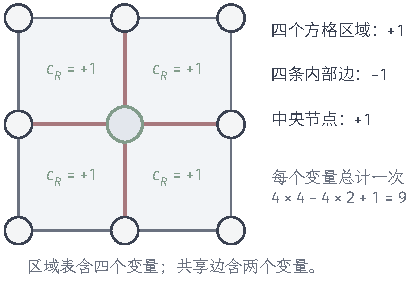
\includegraphics[width=70.831mm]{figures/06-probabilistic-graphical-models/02-inference/tikz/pgm-variational-regions/figure.pdf}
  \caption{四方格区域近似的计数。浅色块表示四个计数为$+1$的四变量区域，粗线标出四个计数为$-1$的共享内部边区域，中央节点区域的计数为$+1$。外边界线是原网格边，不表示本构造额外维护了外边界区域。每条区域一致性约束都要求大表格向子区域边缘化后与小表格相同；颜色之外还用区域面积、线条和节点区分三个层次。}
  \label{fig:pgm-variational-regions}
\end{figure}

区域消息可以由自由能的约束驻点条件导出。对约束$\sum_{\bm z_{R\setminus S}}b_R-b_S=0$引入乘子$\lambda_{R,S}(\bm z_S)$。对某张$b_R$求导时，$R$作为父区域产生正的出边乘子，作为子区域产生负的入边乘子；将它们移到等式右侧，内部驻点满足
\begin{equation}
  c_R(\log b_R-\Theta_R)
    =\sum_{P:\,P\to R}\lambda_{P,R}
       -\sum_{S:\,R\to S}\lambda_{R,S}+\text{常数}.
  \label{eq:pgm-variational-region-stationarity}
\end{equation}
归一化项及$c_R$带来的常数已经合并。每个乘子都是子区域配置上的函数，用来协调父、子两张表；因此它的指数可以作为正的校正因子。不过，直接指数化这里的$\lambda_{R,S}$，通常不能得到下面标准父子形式中的同名边消息，因为驻点方程还含$c_R$，同一约束也可能有冗余表示。需要先把一致性约束重新组合，再给新乘子取指数。消息以整个子区域的配置为索引，负计数区域的校正还会在更新中产生分母，计算对象因此比单节点消息更大。$c_R=0$时，上式只给出乘子之间的约束，不能除以$c_R$来求$b_R$；这一约束及原有的边缘一致性都应保留。

为说明计数怎样进入这种重组，记$\mathcal A(R)$为$R$的严格祖先集合，$b_A^{\downarrow S}$为将$b_A$向$S$边缘化所得的表。对一条父子边$P\to S$，考察加权约束
\begin{equation}
  G_{P,S}:=c_Sb_S+
    \sum_{A\in\mathcal A(S)\setminus(\{P\}\cup\mathcal A(P))}
         c_A b_A^{\downarrow S}=0.
  \label{eq:pgm-variational-region-weighted-constraint}
\end{equation}
原有的逐边一致性保证其中每张祖先表都边缘化为$b_S$。又因为区域及其全部祖先的计数之和为$1$，将$S$与$P$的这两个计数恒等式相减，便得
\[
  c_S+
    \sum_{A\in\mathcal A(S)\setminus(\{P\}\cup\mathcal A(P))}
      c_A=0.
\]
因此$G_{P,S}=0$确实是原一致性约束的线性组合。在四方格例中，边区域$S=e_{A,B}$只有两个祖先$A,B$，而$c_S=-1,c_A=c_B=1$，所以$G_{A,S}=0$就是$-b_S+b_B^{\downarrow S}=0$，$G_{B,S}=0$则是$-b_S+b_A^{\downarrow S}=0$。两条约束交换了原来分别协调的父区域，负计数已包含在这个组合中。

在当前四方格这种所有保留区域计数均非零的有效构造中，还能反向恢复原一致性。具体地，从最大区域向下归纳，设当前子区域$S$上方的表已经一致，记$v_S=c_Sb_S+\sum_{A\in\mathcal A(S)}c_A b_A^{\downarrow S}$。对任一父区域$P$，$P$及其祖先的计数和为$1$，而相应表已与$b_P$一致，所以$G_{P,S}=0$给出$v_S=b_P^{\downarrow S}$。各父表在$S$上的边缘因而相同，所有祖先的边缘也都等于$v_S$。将这一结果代回$v_S$的定义，得到$v_S=c_Sb_S+(1-c_S)v_S$；由$c_S\ne0$即得$b_S=v_S=b_P^{\downarrow S}$。重组约束因而不改变这些表所需满足的边缘关系。

为把这些约束写成消息，记$\mathcal D(R)$为$R$及其全部后代，$\partial R$为所有从$\mathcal D(R)$外进入$\mathcal D(R)$的有向区域边。在每个子区域配置上，以$-\xi_{P,S}(\bm z_S)$作为$G_{P,S}=0$的乘子。一个$G_{P,S}$含$b_R$，恰好意味着$S=R$，或$S$是$R$的后代而$P$在$\mathcal D(R)$外；其中$b_R$的系数都是$c_R$。因此，对非零计数区域$R$求导，约束项的贡献为$-c_R\sum_{(P\to S)\in\partial R}\xi_{P,S}$，既包括进入$R$的边，也包括从外部进入其后代的边。将它与自由能导数合并并除以$c_R$，驻点条件就写成$\log b_R=\Theta_R+\sum_{\partial R}\xi_{P,S}+\text{常数}$。取$m_{P\to S}=e^{\xi_{P,S}}$，才得到下面的边界消息表示。

含零计数区域时，上面的反推步骤不能除以$c_S$，加权约束也可能退化，故仍须保留原父子一致性，并由父表边缘确定这些区域的表；有多个父区域时，还要检查它们给出的边缘相同。不能从一条除以零的驻点式定义零计数表。一般有效区域图的父子参数化与驻点关系见Yedidia等人\scite{pgm-variational-yedidia2005}。

在标准父子区域参数化中，还能把消息方程写成可直接计算的形式。令$\Psi_R=e^{\Theta_R}$，伪边缘写为
\[
  b_R(\bm z_R)\propto
    \Psi_R(\bm z_R)
       \prod_{(P\to Q)\in\partial R}m_{P\to Q}(\bm z_Q).
\]

这里$\partial R$中的每条边都终止于$R$或其某个子区域，故相应消息只依赖$\bm z_R$内的变量。例如，四方格区域图只连接方格到其内部边、内部边到中央点。对$R=A$及$S=e_{A,B}$，后代集合及外部入边分别为
\[
  \begin{aligned}
    \mathcal D(A)&=\{A,e_{A,B},e_{A,C},o\},\\
    \partial A&=\{B\to e_{A,B},\ C\to e_{A,C},\\
              &\qquad e_{B,D}\to o,\ e_{C,D}\to o\},\\
    \mathcal D(S)&=\{S,o\},\\
    \partial S&=\{A\to S,\ B\to S,\ e_{A,C}\to o,\\
              &\qquad e_{B,D}\to o,\ e_{C,D}\to o\}.
  \end{aligned}
\]
例如$e_{B,D}\to o$进入了$A$的后代中央点，虽然没有直接进入$A$，仍须出现在$b_A$中。这些入边组合承担了计数校正，不能只保留直接指向当前区域的消息。

再把消息表示代入父子一致性。设$C_R,C_S>0$分别为两张表的归一化常数，则
\[
  \frac{1}{C_R}\sum_{\bm z_{R\setminus S}}
        \Psi_R\prod_{\partial R}m
    =\frac{1}{C_S}\Psi_S\,m_{R\to S}
        \prod_{\partial S\setminus\{R\to S\}}m.
\]
将除$m_{R\to S}$以外的子区域项移到分母，且将与$\bm z_S$无关的$C_S/C_R$吸收到消息归一化中，得到更新方程
\begin{equation}
  m_{R\to S}(\bm z_S)\propto
  \frac{\displaystyle
    \sum_{\bm z_{R\setminus S}}
      \Psi_R(\bm z_R)
       \prod_{(P\to Q)\in\partial R}m_{P\to Q}(\bm z_Q)}
  {\displaystyle
    \Psi_S(\bm z_S)
       \prod_{\substack{(P\to Q)\in\partial S\\(P\to Q)\ne(R\to S)}}
          m_{P\to Q}(\bm z_Q)}.
  \label{eq:pgm-variational-gbp}
\end{equation}

同时出现在分子、分母且只依赖$\bm z_S$的项可先约去；若还依赖被求和的变量，就不能移出求和号约去。上面的四方格例中，$m_{B\to S}$、$m_{e_{B,D}\to o}$及$m_{e_{C,D}\to o}$在两边公共，且都只依赖$S$内的变量，所以更新可化为
\[
  m_{A\to S}(\bm z_S)\propto
     \frac{\displaystyle\sum_{\bm z_{A\setminus S}}
          \Psi_A(\bm z_A)
          m_{C\to e_{A,C}}(\bm z_{e_{A,C}})}
          {\Psi_S(\bm z_S)m_{e_{A,C}\to o}(z_o)}.
\]
分母中的中央点消息正是为避免重复计入其余重叠区域而保留的校正。消息用正值初始化，每次在父区域求和、在子区域上比较并归一化，然后继续更新其他区域。这就是\term{广义置信传播}（generalized belief propagation, GBP）的一种父子消息形式。这一参数化以覆盖、计数和连通条件为前提；不同冗余约束与消息规范会给出不同但相关的更新式。固定点关系和算法构造的完整论述见Yedidia等人\scite{pgm-variational-yedidia2005}。

对贯穿例子，只要把三变量三角形本身选为最大区域，就需维护$8$项的表格；区域自由能退化为整个联合分布的真实自由能，最优值恰为$-\log26$。整个三角形区域保留了例子中的全部依赖，但也需要存储完整联合表格。若每个变量有$k$个状态，大小为$r$的区域需要$k^r$项，交集一致性还带来额外存储与通信。一般图上不断加入区域未必单调改善Kikuchi目标或每个边缘的误差，因为熵近似也随区域选择改变。满足运行交集性质的精确团树等特殊区域结构，可以建立全局一致性；一般区域图的自由能凸性和GBP收敛则需要分别分析。

区域扩张同时改变伪边缘及其一致性约束；另一条路线保持成对局部多面体不变，改用树分布构造可控的熵近似。以下仍是有限离散成对模型，先设原图连通。选取一族生成树，令参与求和的每棵树$T$都有权重$\rho_T>0$且$\sum_T\rho_T=1$；没有选入的树等价于权重为$0$。为使每条原图边都参与树熵，本节所选树族覆盖全部边。记$\rho_{i,j}=\sum_{T:(i,j)\in T}\rho_T$为边$(i,j)$的出现率，即按树权重随机选一棵树时该边被选中的概率。不连通图可按各连通分量应用同一构造，或等价地使用覆盖各分量的生成森林。

此处的目标仍是累计所有配置的概率质量，因此要在期望得分之外保留熵。若给熵乘一个系数$\tau>0$，通常称为正温度的目标；当前对数配分函数采用$\tau=1$，后面的配置推断才讨论$\tau\downarrow0$时熵消失的情形。在这个口径下，\term{树重加权}（tree-reweighted, TRW）熵定义为
\begin{equation}
  \begin{aligned}
    H_{\mathrm{TRW}}(\bm b)
      &=\sum_iH(b_i)-\sum_{(i,j)\in E}\rho_{i,j}I(b_{i,j}),\\
    I(b_{i,j})
      &=\sum_{k,l}b_{i,j}(k,l)
            \log\frac{b_{i,j}(k,l)}{b_i(k)b_j(l)}.
  \end{aligned}
  \label{eq:pgm-variational-trw-entropy}
\end{equation}
这里$I$是两节点的互信息，比较同一条边的联合表$b_{i,j}$与其两个节点边缘的乘积。以三角图为例，三棵生成树各取$1/3$权重，每条边在其中两棵树中出现，故$\rho_{i,j}=2/3$；这些系数来自一个共同的树分布。

每棵树的熵为$\sum_iH(b_i)-\sum_{(i,j)\in T}I(b_{i,j})$，所以$H_{\mathrm{TRW}}$是树熵的凸组合。对任意全局$q$，给定其树边缘的最大熵树分布的熵不小于$H(q)$；逐树加权便得$H(q)\leq H_{\mathrm{TRW}}(\bm b(q))$。因此
\begin{equation}
  A(\bm{\theta})\leq
    \max_{\bm b\in\mathcal L}
       \{\langle\bm{\theta},\bm b\rangle+H_{\mathrm{TRW}}(\bm b)\}.
  \label{eq:pgm-variational-trw-partition}
\end{equation}

树熵在树的局部一致边缘上是凹函数，可由根节点熵加沿树条件熵之和看出；其凸组合仍凹。因此这是凹目标的凸约束最大化。熵上界的依据是树熵的凸组合，边出现率因此需要来自一个树分布。关于配分函数上界的原始构造见Wainwright等人\scite{pgm-variational-wainwright2005partition}。

成对图的Bethe熵将每条边的互信息减去一次。在含环图上，这组系数通常无法成为生成树分布的边出现率，因此上述树熵上界论证不适用。TRW控制的是最优配分函数目标值，其边缘误差仍需单独检查。TRW用树熵的凸组合获得可控上界，Kikuchi用更大区域加强局部依赖约束；两者改变的机制不同。

\subsubsection{基于矩匹配的近似}

\label{sec:pgm-variational-ep}

前面的平均场/Bethe都在\emph{限制变量依赖或放松一致性}，期望传播（EP）则换了一个出发点：当模型里有一两个特别难处理的因子时，先用一个好算的“替身因子”代替它，得到一个整体好算的近似$q$；然后\emph{轮流}把每个真实因子临时放回去、算出它对关键矩（均值、方差）的影响，再调整替身，使近似分布能\emph{匹配这些矩}。这个“移除替身、放回真因子、匹配矩、写回替身”的循环就是EP。除了限制变量依赖，也可以用容易计算的分布匹配目标的局部特征。若难处理的因子使完整密度的计算成本过高，可以用易计算的指数族因子替代它们。每次暂时恢复一个真实因子，计算它对重要矩的影响，再将这些矩纳入近似分布。

设目标$p(\bm z)\propto p_0(\bm z)\prod_a f_a(\bm z)$，其中$p_0$容易处理，近似取$q(\bm z)\propto p_0(\bm z)\prod_a\widetilde f_a(\bm z)$。站点$\widetilde f_a$是替代真实因子$f_a$的指数族因子，不必单独归一化。若直接将$f_a$乘入当前$q$，真实因子与它的近似替身就会同时出现，相当于重复计入同一份作用。因此先除去$\widetilde f_a$，再放回$f_a$，得到仅在这一处恢复真实因子的临时分布。计算这个分布的均值、方差等所需矩，再寻找能够复现这些矩的近似分布，最后将修正写回站点。\term{期望传播}（expectation propagation, EP）依次在各站点重复这一过程；下面四行分别对应移除、恢复、投影和写回：
\begin{equation}
  \begin{aligned}
    q^{\setminus a}(\bm z)&\propto q(\bm z)/\widetilde f_a(\bm z),\\
    \widehat p_a(\bm z)&=
       \frac{f_a(\bm z)q^{\setminus a}(\bm z)}{Z_a},\\
    q^{\mathrm{new}}&=
       \argmin_{q'\in\mathcal Q}
           \operatorname{KL}(\widehat p_a\Vert q'),\\
    \widetilde f_a^{\mathrm{new}}(\bm z)&\propto
       q^{\mathrm{new}}(\bm z)/q^{\setminus a}(\bm z).
  \end{aligned}
  \label{eq:pgm-variational-ep}
\end{equation}
移除当前近似站点后的$q^{\setminus a}$称为\term{空腔分布}（cavity distribution），它避免同一因子被重复计算；放回真实因子得到的$\widehat p_a$称为\term{倾斜分布}（tilted distribution）。这一更新要求空腔与倾斜分布可归一化，所匹配的矩存在。$Z_a$归一化的是本次倾斜分布。第三行的有限KL投影还要求支持相容、至少一个候选的KL有限，以及最小值在候选族中取得。

具体地，设$q'_{\bm{\lambda}}=h\exp\{\langle\bm{\lambda},\bm T\rangle-A_q(\bm{\lambda})\}$具有固定支持，$\widehat p_a$不在$h=0$处放置质量，$\mathbb E_{\widehat p_a}\lVert\bm T\rVert_2<\infty$。选取一个满足$\operatorname{KL}(\widehat p_a\Vert q'_{\bm{\lambda}_0})<\infty$的候选，便有
\[
  \begin{aligned}
    \operatorname{KL}(\widehat p_a\Vert q'_{\bm{\lambda}})
      ={}&\operatorname{KL}(\widehat p_a\Vert q'_{\bm{\lambda}_0})\\
       &+A_q(\bm{\lambda})-A_q(\bm{\lambda}_0)\\
       &-\langle\bm{\lambda}-\bm{\lambda}_0,
                  \mathbb E_{\widehat p_a}\bm T\rangle.
  \end{aligned}
\]
有限矩使两个候选的对数密度比可积，因此该差值表示可由有限KL候选推得。

在自然参数域内部，按式~\eqref{eq:pgm-variational-moments}对目标求导，得到
\begin{equation}
  \mathbb E_{q^{\mathrm{new}}}\bm T
     =\mathbb E_{\widehat p_a}\bm T.
  \label{eq:pgm-variational-moment-matching}
\end{equation}
在这些有限KL条件下，投影才等价于矩匹配。若目标矩在正则最小指数族的内部均值域中，严格凸性给出唯一的投影参数；若落在边界，可能只能取极限。

矩存在且可实现时，式~\eqref{eq:pgm-variational-moment-matching}可以定义矩匹配更新。若全部候选的KL均为无穷大，该更新仍有矩匹配含义，却缺少有限KL投影解释；矩不存在时，更新本身也无定义。对高斯族，充分统计量是$\bm z$及$\bm z\bm z^\top$，故需匹配均值和协方差。

一维例子可完整算出一次更新。令$p_0(z)=\mathcal N(z;0,1)$，只有一个因子$f(z)=\mathbb I[z\geq0]$，初始近似站点为$1$。此时$q=p_0$，除去常数站点后的空腔仍是标准正态。记其密度为$\varphi(z)=(2\pi)^{-1/2}e^{-z^2/2}$，放回真实因子便将它截在非负半轴上；由对称性，半轴质量$Z_a=\int_0^\infty\varphi(z)\,dz=1/2$，故倾斜密度为$2\varphi(z)\mathbb I[z\geq0]$，即半正态分布。在它的支持上，与标准正态的密度比恒为$2$，所以两者的KL为$\log2<\infty$，满足上述有限性条件。

为求投影高斯，需要先计算两个矩。由$\varphi'(z)=-z\varphi(z)$，有$\int_0^\infty z\varphi(z)\,dz=\varphi(0)$，所以倾斜分布的均值为$2\varphi(0)=\sqrt{2/\pi}$。标准正态的$z^2\varphi(z)$是偶函数，全空间积分为$1$，因此半轴积分为$1/2$，倾斜分布的二阶矩恰为$1$。从二阶矩减去均值平方，得到
\[
  Z_a=\frac12,\qquad
  \mathbb E_{\widehat p_a}Z=\sqrt{\frac2\pi},\qquad
  \operatorname{Var}_{\widehat p_a}(Z)=1-\frac2\pi.
\]
于是$q^{\mathrm{new}}=\mathcal N(m,v)$，$m\approx0.797885$、$v\approx0.363380$。写回站点要用新高斯除以空腔。两者的对数密度分别含$-z^2/(2v)+(m/v)z$和$-z^2/2$，相减后得
\[
  \log\widetilde f_a^{\mathrm{new}}(z)
      =-\frac12(v^{-1}-1)z^2+\frac{m}{v}z+\text{常数}.
\]
若高斯自然参数写成$\eta z-\tau z^2/2$，新站点参数因此为$\tau_a=v^{-1}-1$、$\eta_a=m/v$。站点与空腔重新相乘，恰好恢复投影所得的$q^{\mathrm{new}}$。该高斯匹配均值和方差，同时在$z<0$处保留正概率。将它用于反向$\operatorname{KL}(q\Vert p)$时，目标的硬支持使KL为无穷大。矩匹配与反向KL由此对支持施加了不同要求。

EP每次投影的$\widehat p_a$依赖其他近似站点，所以其局部投影目标也随迭代变化。固定点可以与特定自由能的驻点联系起来，普通站点更新的单调性和收敛性则需要另外分析。高斯站点是不归一化的指数族因子，其精度允许为负；总体$q$以及实际使用的空腔和倾斜分布仍需合法。计算中可以采用自然参数阻尼，并检查协方差正定性和矩匹配残差。EP的站点替换与矩匹配构造来自Minka\scite{pgm-variational-minka2001}。

\subsubsection{基于局部曲率的近似}

\label{sec:pgm-variational-laplace}

对连续后验，还有一个最简单直观的近似：如果后验的质量主要集中在一个光滑的峰附近，那它在峰附近看起来就很像一个高斯——只需知道\emph{峰在哪里}（众数）和\emph{峰有多陡}（众数处的曲率，即负Hessian），就能完全确定这个高斯。拉普拉斯近似因此不需要迭代积分，只要做一次优化求众数、再算一次二阶导数。与逐因子修正的EP并行，若连续后验的主要质量集中在一个光滑峰附近，可以直接近似整个对数密度的局部形状。\term{拉普拉斯近似}（Laplace approximation）在众数附近作二阶展开，用峰的位置和曲率决定一个高斯。令$\ell(\bm z)=\log p(\bm x,\bm z)$，$\widehat{\bm z}$是内部严格局部极大点，且$\bm H=-\nabla^2\ell(\widehat{\bm z})$正定，则
\begin{equation}
  \begin{aligned}
    \ell(\bm z)&\approx\ell(\widehat{\bm z})
       -\frac12(\bm z-\widehat{\bm z})^\top
                  \bm H(\bm z-\widehat{\bm z}),\\
    q_{\mathrm L}(\bm z)&=\mathcal N(\widehat{\bm z},\bm H^{-1}),\\
    p(\bm x)&\approx
       e^{\ell(\widehat{\bm z})}(2\pi)^{d/2}|\bm H|^{-1/2}.
  \end{aligned}
  \label{eq:pgm-variational-laplace}
\end{equation}
线性项因众数处梯度为零而消失，高斯积分产生行列式项。计算上需要求众数、计算Hessian，再用Cholesky分解求解线性系统及对数行列式，不必显式求逆。负Hessian存在零方向或负方向时，上述协方差无法定义。强制正定的曲率修正可以得到其他高斯近似，但已改变原始二阶展开。

以Gamma密度$p(z)\propto z^{a-1}e^{-bz}$、$z>0$为例，取$a>1,b>0$。与$z$有关的对数密度为$\ell(z)=(a-1)\log z-bz+\text{常数}$，其两阶导数为
\[
  \ell'(z)=\frac{a-1}{z}-b,\qquad
  \ell''(z)=-\frac{a-1}{z^2}.
\]
令一阶导数为零，得到内部众数$\widehat z=(a-1)/b$；代入负二阶导数，得$-\ell''(\widehat z)=b^2/(a-1)>0$，取倒数便是近似方差。因此拉普拉斯近似为$\mathcal N((a-1)/b,(a-1)/b^2)$。当$a=3,b=1$时，它的均值、方差为$2,2$，而Gamma真实值分别为$a/b=3$、$a/b^2=3$。记标准正态分布函数为$\Phi$，近似高斯落在非法负半轴的质量为$\Phi((0-2)/\sqrt2)=\Phi(-\sqrt2)\approx7.865\%$。这里的偏差来自众数不等于均值、曲率不等于整体方差，以及二阶展开没有保留支持边界。

若改用$y=\log z$，则$z=e^y$且$dz/dy=e^y$，必须把Jacobian计入新坐标的密度：
\[
  p_Y(y)=p_Z(e^y)e^y
       \propto e^{(a-1)y-be^y}e^y
       =\exp(ay-be^y).
\]
正是Jacobian的$e^y$将对数密度中$y$的系数从$a-1$改为$a$。新对数密度的一阶导数为$a-be^y$，二阶导数为$-be^y$，故众数为$\widehat y=\log(a/b)$，众数处负曲率为$a$，近似为$Y\sim\mathcal N(\log(a/b),1/a)$。变回$Z=e^Y$便得到对数正态近似，保证正支持，却不等于直接在$z$坐标中得到的高斯。因此，拉普拉斯近似依赖展开所用的坐标；保留Jacobian后，坐标变换同时改变近似的形状和支持。

局部二阶展开近似整个积分，还需要主峰支配和尾部可控。若$\ell_n$随样本量$n$集中，唯一主峰附近的曲率按$n$增长，且高阶导数与尾部满足相应正则性，拉普拉斯法可给出渐近展开。有限样本误差则取决于峰外质量、偏斜和尾部等性质。单个高斯会遗漏其他模态；将多个峰的贡献相加时，需要找到相关峰并避免重复计数。拉普拉斯法依据局部曲率构造近似，一般没有ELBO最优性或证据上下界保证\scite{bishop2006}。

\subsection{近似的计算}
\label{sec:pgm-variational-stochastic-amortized}
\label{sec:pgm-variational-complexity}

\label{sec:pgm-variational-scalable}
选定近似族后，还要把更新公式变成可执行的计算，需处理四类问题：平均场坐标更新中的期望何时能\emph{闭式}算出（条件共轭，对应VMP）；全局参数每更新一次都要\emph{遍历全部}$n$个样本时如何降低成本（小批量的随机变分推断SVI）；ELBO中的期望积不出来时梯度如何估计（重参数化与分数函数两种梯度）；每来一个新样本都重新优化后验过于重复时如何复用（摊销推断，用共享网络一次给出后验）。下面先利用局部结构计算更新，再降低数据遍历成本，随后处理难解期望的梯度，最后减少新观测的重复优化；满足各自条件时，这些方法可以组合使用。

\subsubsection{计算局部更新}

\label{sec:pgm-variational-coordinate-vmp}
\label{sec:pgm-variational-vmp}

式~\eqref{eq:pgm-variational-coordinate}虽然形式简洁，指数中的期望仍可能难算。若完整条件分布属于指数族，
\[
  \log p(z_i\mid\bm{z}_{-i},\bm{x})
    =\log h_i(z_i)
      +\langle\bm{\eta}_i(\bm{z}_{-i},\bm{x}),\bm T_i(z_i)\rangle
      +c(\bm{z}_{-i},\bm{x}),
\]
且相关期望存在，则更新后的$q_i$保持同一家族，自然参数为
\begin{equation}
  \bm{\lambda}_i
    =\mathbb E_{q_{-i}}\bm{\eta}_i(\bm{Z}_{-i},\bm{x}).
  \label{eq:pgm-variational-conjugacy}
\end{equation}
这一结论可直接从坐标更新看出。完整条件分布与联合分布的对数只相差一个不依赖$z_i$的项，代回式~\eqref{eq:pgm-variational-coordinate}后，便得到
\[
  \log q_i^{\mathrm{new}}(z_i)
    =\log h_i(z_i)
      +\left\langle\mathbb E_{q_{-i}}\bm\eta_i,
                       \bm T_i(z_i)\right\rangle+c_i^{\mathrm{norm}},
\]
其中$c_i^{\mathrm{norm}}$只负责归一化。因此，取期望改变的是$\bm T_i$前面的自然参数，不改变关于$z_i$的函数形式。这就是条件共轭带来的计算闭合。这里不要求$\bm{\eta}_i$对其他变量线性，但必须能够计算其期望，并确认结果落在合法自然参数域内；一般不能用$\bm\eta_i(\mathbb E\bm Z_{-i},\bm x)$代替$\mathbb E\bm\eta_i(\bm Z_{-i},\bm x)$。

在因子图中，设每个邻接因子的对数中与$z_i$有关的部分能写成$\langle\bm{\eta}_{a\to i}(\bm z_{S_a\setminus\{i\}}),\bm T_i(z_i)\rangle$。把$\log h_i$只计入一次，定义消息
\[
  \bm m_{a\to i}
    =\mathbb E_{q_{S_a\setminus\{i\}}}\bm{\eta}_{a\to i},
  \qquad
  \bm{\lambda}_i=\sum_{a:\,i\in S_a}\bm m_{a\to i}.
\]
在标准共轭构造中，局部自然参数对邻居的充分统计量具有可分解的形式。例如，若某个贡献为不同邻居的$T_j(z_j)T_k(z_k)$，平均场独立性使其期望等于$\mathbb E_{q_j}T_j\,\mathbb E_{q_k}T_k$。因此变量可以把$\mathbb E_{q_i}\bm T_i$发给邻接因子，由因子组合这些期望，得到下一次所需的自然参数消息。这里需要检查的是这些统计量是否足以完成当前期望计算。若$\bm\eta_{a\to i}$包含未被所传统计量覆盖的非线性函数，就还需计算相应的高阶矩，或根据已知的$q_j$形式进行额外积分；只发送均值不会自动使任意非线性期望可算。

\term{变分消息传递}（variational message passing, VMP）就是这种利用局部结构、以所需充分统计量和自然参数交换实现坐标优化的方式。消息不必是归一化概率表，也不同于和积算法对原因子先乘后求和的消息。闭式VMP利用所选因子化及条件共轭求出期望；非共轭模型则需结合局部界、数值积分或梯度更新完成这一计算\scite{pgm-variational-winn2005}。

例如，全局成功率$\Pi\sim\operatorname{Beta}(a_0,b_0)$，$Z_i\mid\Pi\sim\operatorname{Bernoulli}(\Pi)$，观测因子为$p(x_i\mid z_i)$。取$q(\pi)\prod_iq_i(z_i)$，记$r_i=q_i(Z_i=1)$。先更新$q(\pi)$，与$\pi$有关的期望对数联合项为
\[
  \left(a_0-1+\sum_i r_i\right)\log\pi
   +\left(b_0-1+\sum_i(1-r_i)\right)\log(1-\pi).
\]
这正是Beta密度的两个对数项，说明成功与失败的整数计数被软计数替代。再更新$q_i$时，把$z_i=1$与$z_i=0$的期望对数得分相减，先验部分给出$\mathbb E\log\Pi-\mathbb E\log(1-\Pi)$，观测部分给出对数似然比。因此
\begin{equation}
  \begin{aligned}
    q(\pi)&=\operatorname{Beta}(a,b),\\
    a&=a_0+\sum_i r_i,\qquad
    b=b_0+\sum_i(1-r_i),\\
    \log\frac{r_i}{1-r_i}
      &=\mathbb E_q\log\Pi-\mathbb E_q\log(1-\Pi)
         +\log\frac{p(x_i\mid1)}{p(x_i\mid0)}.
  \end{aligned}
  \label{eq:pgm-variational-beta-bernoulli}
\end{equation}
其中$\mathbb E\log\Pi=\psi(a)-\psi(a+b)$、$\mathbb E\log(1-\Pi)=\psi(b)-\psi(a+b)$，$\psi(u)=d\log\Gamma(u)/du$是双伽马函数。局部变量向全局因子发送的是软计数$(r_i,1-r_i)$，全局变量返回的是期望对数概率，而不是$\log\mathbb E\Pi$。

取$a_0=b_0=1$，两个样本的似然比分别为$4$和$1/4$。从$q(\pi)=\operatorname{Beta}(1,1)$开始，局部更新给出$r_1=0.8,r_2=0.2$；全局更新得到$\operatorname{Beta}(2,2)$。由于新的两个期望对数概率仍相等，再次局部更新不变。这次更新通过两个软计数和两个期望完成，避免枚举$(Z_1,Z_2,\Pi)$的联合状态。相应的表达代价是$q$将$\Pi$与各$Z_i$独立化，丢失它们的后验相关性。

近似方法的单轮成本取决于需要存储和更新的局部对象。设有限离散成对图有$d$个节点、$m$条边，每节点至多$k$个状态。存储一般的稠密边势需$O(mk^2)$。一次完全平均场扫描在直接计算全部边期望时通常需$O(mk^2)$，变分边缘本身只需$O(dk)$空间；Ising等特殊代数结构可以更快。一次成对LBP扫描也通常需$O(mk^2)$，但需要$O(mk)$条目保存有向消息，若显式保存边伪边缘则另需$O(mk^2)$。在这一稠密成对设定下，两者单轮成本量级相近；总成本还取决于迭代轮数，近似误差还取决于所保留的依赖。

对于作用域$S_a$的稠密高阶因子，单次朴素局部求和本身就可能涉及$k^{|S_a|}$个配置。VMP可利用充分统计量期望的简洁形式减少枚举，其实际代价取决于这些期望的计算方式。块变分若内部树宽为$w$，表格推断通常带有$k^{w+1}$因子；Kikuchi最大区域有$r$个变量时，至少要面对$k^r$级区域表。区域方法的通信按交集状态数增长，增加区域既增加局部成本，也增加一致性校正工作。

连续近似的瓶颈常在矩阵运算。一个$d$维稠密高斯的协方差需要$O(d^2)$空间，通用Cholesky分解需$O(d^3)$时间；拉普拉斯近似与高斯EP都可能遇到它。稀疏精度、低秩更新、分块或对角表示能改变实际代价，但也可能改变近似族。EP若每个站点作用于低维投影，可局部计算倾斜矩并利用低秩更新；此时一次站点替换的代价由局部矩计算和低秩更新决定。

\subsubsection{降低数据遍历成本}

\label{sec:pgm-variational-svi}

即使每个局部更新便宜，遍历全部$n$个样本才能改变一次全局参数，也会拖慢大数据推断。设全局潜变量为$\bm u$，样本局部潜变量为$\bm z_i$，
\[
  p(\bm u,\bm z_{1:n},\bm x_{1:n})
    =p(\bm u)\prod_{i=1}^n p(\bm x_i,\bm z_i\mid\bm u),
  \qquad
  q=q_{\bm{\lambda}}(\bm u)\prod_iq_{\bm{\phi}_i}(\bm z_i).
\]
假设共轭使全局完整条件分布的自然参数等于$\bm{\lambda}_0+\sum_i\bm s(\bm x_i,\bm z_i)$。其中$\bm\lambda_0$来自先验，$\bm s_i=\bm s(\bm x_i,\bm z_i)$是第$i$个样本对全局参数的统计量贡献。固定局部因子时，最优全局自然参数为$\bm{\lambda}^\star=\bm{\lambda}_0+\sum_i\mathbb E_{q_i}\bm s_i$。

这个最优参数还给出一个适合随机更新的方向。为看清方向的来源，把全局近似写为
\[
  \log q_{\bm\lambda}(\bm u)
    =\log h(\bm u)+\langle\bm\lambda,\bm T(\bm u)\rangle
       -A_q(\bm\lambda).
\]
在固定局部因子后，期望对数联合分布中依赖$\bm u$的项具有同一基准项$\log h$，其统计量系数为$\bm\lambda^\star$。两者相减时，基准项抵消，且$\mathbb E_{q_{\bm\lambda}}\bm T=\nabla A_q(\bm\lambda)$，于是全局ELBO中依赖$\bm{\lambda}$的部分为
\[
  \mathcal L(\bm\lambda)
    =\langle\bm{\lambda}^\star-\bm{\lambda},
            \nabla A_q(\bm{\lambda})\rangle+A_q(\bm{\lambda})+C,
\]
其中$C$不依赖当前全局参数。对内积使用乘积求导，得到
\[
  \begin{aligned}
    \nabla_{\bm\lambda}\mathcal L
      &=-\nabla A_q(\bm\lambda)
        +\nabla^2 A_q(\bm\lambda)(\bm\lambda^\star-\bm\lambda)
        +\nabla A_q(\bm\lambda)\\
      &=\nabla^2 A_q(\bm\lambda)(\bm\lambda^\star-\bm\lambda).
  \end{aligned}
\]
两个一阶矩项抵消，剩下的Hessian来自矩对参数的变化率。

普通欧氏梯度以参数坐标的距离衡量更新大小，但相同长度的参数改动，可能引起不同程度的分布变化。在最小、正则指数族的自然参数域内部，Fisher信息矩阵为$\bm F(\bm\lambda)=\nabla^2 A_q(\bm\lambda)$，且正定。对于足够小的参数改动$\Delta\bm\lambda$，局部KL的二阶项为$\tfrac12\Delta\bm\lambda^\top\bm F(\bm\lambda)\Delta\bm\lambda$，所以$\bm F$给出了分布变化的局部尺度。\term{自然梯度}（natural gradient）采用$\widetilde\nabla\mathcal L=\bm F^{-1}\nabla\mathcal L$，按这一尺度校正欧氏梯度。将刚才的普通梯度代入，$\bm F^{-1}$与Hessian抵消，从而
\begin{equation}
  \widetilde\nabla_{\bm{\lambda}}\mathcal L
    =\bm{\lambda}_0+\sum_i\mathbb E_{q_i}\bm s_i-\bm{\lambda}.
  \label{eq:pgm-variational-natural-gradient}
\end{equation}
式~\eqref{eq:pgm-variational-natural-gradient}先对固定局部因子的ELBO成立。若局部因子在其参数域内部达到给定全局参数下的光滑最优值，且局部最优解及优化后的目标满足相应可微条件，包络定理允许用同一偏导计算优化掉局部变量后的目标梯度。其原因是局部最优点处关于局部参数的一阶变化为零，链式求导中由局部解随全局参数移动而产生的项随之消失；局部最优解位于约束边界、解不唯一或最优点处不可微时，需要核对相应的一阶条件与包络条件，不能直接沿用内部驻点处梯度为零的解释。

均匀抽取大小为$b$的小批量$B$，更新其中局部因子后，用
\begin{equation}
  \begin{aligned}
    \widehat{\bm{\lambda}}
      &=\bm{\lambda}_0+\frac{n}{b}
           \sum_{i\in B}\mathbb E_{q_i}\bm s_i,\\
    \bm{\lambda}^{(t)}
      &=(1-\rho_t)\bm{\lambda}^{(t-1)}
          +\rho_t\widehat{\bm{\lambda}}
  \end{aligned}
  \label{eq:pgm-variational-svi}
\end{equation}
构造\term{随机变分推断}（stochastic variational inference, SVI）的全局更新。这里还要保证每一步仍对应合法分布。记$\Omega=\operatorname{int}\{\bm\lambda:A_q(\bm\lambda)<\infty\}$为当前正则族所用的自然参数域，并选取$\bm\lambda^{(0)}\in\Omega$。指数族的自然参数域是凸的；若本批目标$\widehat{\bm\lambda}\in\Omega$，且$0<\rho_t\leq1$，上式便是域内两点的凸组合，因而仍在$\Omega$内。小批量缩放后的目标是否在域内，需要由具体共轭模型确认；若不满足，不能直接使用该次更新，应修正目标的构造或采用另外有合法性保证的更新。对于非凸的其他约束，还需检查这些约束本身。步长大于$1$会变成外推，即使两个端点都合法，也不保证新参数合法。

在给定当前全局参数并精确求解相应局部问题时，缩放的统计量和是全数据和的无偏估计。非均匀抽样需要按纳入概率加权；局部问题未充分求解时，估计中还包含局部优化误差，精确局部解下的无偏结论需要相应调整\scite{pgm-variational-hoffman2013}。

在式~\eqref{eq:pgm-variational-beta-bernoulli}中，若$n=1000$，抽到的$10$个样本的$r_i$之和为$7$，先验仍为$\operatorname{Beta}(1,1)$，则小批量给出的目标分布是$\operatorname{Beta}(701,301)$。若当前分布为$\operatorname{Beta}(501,501)$，取步长$0.1$，更新为$\operatorname{Beta}(521,481)$。缩放发生在统计量而不是先验上，否则会把先验重复计算。

随机更新以有噪声的小批量方向替代全数据方向，因此单步ELBO可能下降。在保持上述每步合法性的基础上，常用递减步长还满足$\sum_t\rho_t=\infty$、$\sum_t\rho_t^2<\infty$。例如，从$t=1$起取$\rho_t=(t+t_0)^{-\kappa}$，其中$t_0\geq0$、$1/2<\kappa\leq1$，就同时有$0<\rho_t\leq1$与这两个和式条件。式~\eqref{eq:pgm-variational-svi}中的当前参数因此记为$\bm\lambda^{(t-1)}$，更新后记为$\bm\lambda^{(t)}$。和式条件约束长期累计的更新及噪声，并不能代替参数域检查。在光滑性、迭代有界、噪声矩受控等随机逼近条件下，可以分析迭代趋向驻点的行为。局部计算解释当前批次的样本，全局计算汇总缩放后的统计量，这一分工使每次更新只需读取部分数据。

SVI将每次全数据局部计算从$n$个样本改为$b$个样本，代价约为$bC_{\mathrm{local}}+C_{\mathrm{global}}$，其中两项分别是单样本局部更新和全局更新成本。若无需保留所有局部因子，还可避免$O(n)$份局部状态存储；总训练成本仍取决于达到目标精度所需的小批量数。

近似族的选择取决于需要估计的量。主要计算单变量边缘且内存有限时，完全平均场提供成本较低的起点；其遗漏的相关性仍可能影响这些边缘。若查询涉及相邻状态的联合概率或整段轨迹，保留链或小块依赖能直接表达所需的联合事件，代价是块内推断。是否增加结构，需要比较相关查询的误差和计算成本。

计算方式可以叠加在选定的近似族上。条件共轭且统计量期望可算时，VMP组织解析更新；模型还具有可分解的局部统计量和全局更新时，SVI通过小批量减少一次遍历的数据量。例如，每个样本是一段序列时，可在$q_{\bm\phi_i}(\bm z_i)$中保留整条链，精确计算链内统计量，再用小批量更新共轭的全局参数。这一组合同时保留局部结构并降低数据遍历成本，单条链内部的推断复杂度仍由链的模型决定。

\subsubsection{估计难解期望的梯度}
\label{sec:pgm-variational-gradient-estimation}

小批量抽样减少了需要处理的数据量，但每个样本的ELBO仍可能包含无法解析计算的期望。非共轭模型中，局部更新因而常需改为梯度优化，并通过潜变量采样估计梯度。困难在于：改变近似参数时，$q$既改变被平均的函数，也改变样本落在哪里。若把已经抽到的样本当成固定输入，只对函数求导，就可能漏掉分布变化的影响。为了保留这一影响，可以先抽取分布固定的噪声，再把噪声变换为$q$的样本；改变参数时，沿同一份噪声追踪样本位置的变化。对于能够写成$\bm z=g_{\bm{\phi}}(\bm\epsilon)$、$\bm\epsilon\sim r(\bm\epsilon)$且$r$不依赖$\bm{\phi}$的分布，随机性可以与参数分开。例如高斯分布可写为$\bm z=\bm m+\bm L\bm\epsilon$，$\bm\epsilon\sim\mathcal N(\bm0,\bm I)$，$\bm L\bm L^\top$为协方差。令$F_{\bm{\phi}}(\bm z)=\log p(\bm x,\bm z)-\log q_{\bm{\phi}}(\bm z)$，当$g_{\bm\phi}$和$F_{\bm\phi}$在所需参数与样本处可微，且链式导数满足可交换微分与期望的可积支配条件时，
\begin{equation}
  \begin{aligned}
    \nabla_{\bm{\phi}}\mathcal L
      =\mathbb E_r\big[
        &(\nabla_{\bm{\phi}}g_{\bm{\phi}})^\top
           \nabla_{\bm z}F_{\bm{\phi}}
                (g_{\bm{\phi}}(\bm\epsilon))\\
        &+\left.\nabla_{\bm{\phi}}F_{\bm{\phi}}(\bm z)
          \right|_{\bm z=g_{\bm{\phi}}(\bm\epsilon)}
        \big].
  \end{aligned}
  \label{eq:pgm-variational-pathwise}
\end{equation}
第二行对$\bm z$保持固定，只微分$F$的显式参数依赖；第一行则跟踪样本位置随参数移动的影响。这是\term{重参数化梯度}（reparameterization gradient），也称路径导数估计：先把期望写到固定噪声上，再用链式法则求导。样本位置的参数依赖由第一项显式保留；模型含待学习参数时，还需计算对应的显式偏导。第~\ref{chap:pgm-generative}章将在VAE中使用这一梯度估计\scite{kingma2013}。

以$q=\mathcal N(m,s^2)$、$s>0$和$f(z)=z^2$为例，$z=m+s\epsilon$，路径导数的单样本估计分别是$2(m+s\epsilon)$与$2(m+s\epsilon)\epsilon$，期望为$2m$与$2s$，恰与$\partial_m(m^2+s^2)$、$\partial_s(m^2+s^2)$一致。这些单样本导数的期望给出正确梯度，但有限样本估计仍有方差。与其他估计器的方差比较，需要固定目标函数和分布。

离散变量的普通采样映射对参数通常是阶梯函数，几乎处处导数为零，直接套用路径导数不能得到正确梯度。另一种办法直接微分概率权重，而不追踪单个样本的位置。为使用这一办法，先假设$q_{\bm\phi}$相对于同一基准测度，在一个不随$\bm\phi$变化的支持集上为正，且$q_{\bm\phi}$与$f_{\bm\phi}$对参数可微。有限状态空间中，可在各项有限时逐项求导；对于可数无穷或连续支持，还需要允许微分与求和或积分交换。例如，在当前参数的一个邻域内，$q_{\bm\phi}f_{\bm\phi}$及$q_{\bm\phi}$的各参数偏导分别受可积函数支配，并且下面乘积求导后的两项均绝对可积，就是一组足够条件。此时，按同一测度积分，有
\[
  \begin{aligned}
    \nabla_{\bm\phi}\int q_{\bm\phi}(\bm z)f_{\bm\phi}(\bm z)\,d\bm z
      &=\int\big[(\nabla_{\bm\phi}q_{\bm\phi})f_{\bm\phi}
                   +q_{\bm\phi}\nabla_{\bm\phi}f_{\bm\phi}\big]\,d\bm z.
  \end{aligned}
\]
再在正支持集上代入$\nabla q=q\nabla\log q$，可得
\begin{equation}
  \nabla_{\bm{\phi}}\mathbb E_{q_{\bm{\phi}}}f_{\bm{\phi}}(\bm Z)
    =\mathbb E_q\!\left[
       f_{\bm{\phi}}(\bm Z)\nabla_{\bm{\phi}}\log q_{\bm{\phi}}(\bm Z)
       +\nabla_{\bm{\phi}}f_{\bm{\phi}}(\bm Z)\right].
  \label{eq:pgm-variational-score-function}
\end{equation}
这称为\term{分数函数估计}（score-function estimator），其中“分数”指对数密度对参数的导数。固定支持排除了移动积分边界的影响，可微性与求导交换条件则支持上面的乘积求导，二者承担不同职责。在同样允许对归一化等式求导的条件下，
\[
  \mathbb E_q\nabla_{\bm\phi}\log q_{\bm\phi}
    =\int\nabla_{\bm\phi}q_{\bm\phi}\,d\bm z
    =\nabla_{\bm\phi}\int q_{\bm\phi}\,d\bm z=\bm0.
\]
因此，从第一项的$f_{\bm\phi}$中减去不依赖所采变量的基线，不改变这一项的期望，却可能降低方差。若基线还依赖参数，这个结论是把它作为该梯度估计器中的系数使用，并不意味着可以把整个目标换成$f_{\bm\phi}$减基线后再忽略其显式导数。小状态空间也可以精确求和；连续松弛则用可微随机变量替代离散变量，一般改变了目标或引入偏差。支持集随参数变化时，求导还涉及积分边界，上式需要加入相应的边界处理。

\subsubsection{降低重复推断成本}

\label{sec:pgm-variational-amortized}

小批量减少了每次读取的数据，却仍需为每个新样本求解局部优化。若样本不断到来，可以学习一个共享映射$\bm{\phi}_i=f_{\bm{\omega}}(\bm x_i)$，直接输出$q_{\bm{\phi}_i}(\bm z_i)$的参数。\term{摊销推断}（amortized inference）把许多样本的推断计算转移到一次共享训练中；测试时主要执行前向计算，也可以在其输出上继续作样本级优化。

摊销推断将测试时的迭代换成网络前向计算，共享训练还需计入反向传播和模型存储。小批量SVI与摊销映射可以结合：每次只抽取一批样本，用共享映射生成它们的局部参数，再计算这一批的统计量或梯度。小批量减少每次处理的数据量，摊销映射减少每个样本单独执行的优化；网络输出若未达到局部最优，仍须保留前述局部优化误差的限制。

共享映射减少了逐样本优化，也限制了各样本的局部参数如何取值。为分解其逐样本误差，以下改用固定生成参数$\bm\theta$、样本间相互独立的局部潜变量模型，并定义局部ELBO：
\[
  \begin{aligned}
    p_{\bm\theta}(\bm x_{1:n},\bm z_{1:n})
      &=\prod_i p_{\bm\theta}(\bm x_i,\bm z_i),\\
    \mathcal L_i(\bm\phi)
      &=\mathbb E_{q_{\bm\phi}}
          \log p_{\bm\theta}(\bm x_i,\bm Z_i)+H(q_{\bm\phi}).
  \end{aligned}
\]
前面的SVI层次模型包含共享随机量$\bm u$，积分掉它通常产生样本间依赖，联合对数证据因而不能逐样本相加，其ELBO还包括全局因子的贡献。

在上述独立模型中，令$\mathcal L_i^\star=\sup_{\bm{\phi}}\mathcal L_i(\bm{\phi})$；设共享网络达到其最优参数$\bm{\omega}^\star$，实际训练结果为$\widehat{\bm{\omega}}$。假设以下各目标值有限，对同一批样本有
\begin{equation}
  \begin{aligned}
    &\sum_i\log p_{\bm\theta}(\bm x_i)
       -\sum_i\mathcal L_i(f_{\widehat{\bm{\omega}}}(\bm x_i))\\
    ={}&\sum_i[\log p_{\bm\theta}(\bm x_i)-\mathcal L_i^\star]\\
     &+\left[\sum_i\mathcal L_i^\star
          -\sum_i\mathcal L_i(f_{\bm{\omega}^\star}(\bm x_i))\right]\\
     &+\left[\sum_i\mathcal L_i(f_{\bm{\omega}^\star}(\bm x_i))
          -\sum_i\mathcal L_i(f_{\widehat{\bm{\omega}}}(\bm x_i))\right].
  \end{aligned}
  \label{eq:pgm-variational-amortization-gap}
\end{equation}
三项分别是近似族误差、共享映射限制带来的摊销误差和网络优化误差，按定义均非负。若最优值未取得，改用上确界解释。网络最优性针对同一固定模型下的样本总目标，个别样本上的ELBO可能低于实际训练结果。关于近似与摊销两类误差的区分，可参见Cremer等人的分析\scite{pgm-variational-cremer2018}。

式~\eqref{eq:pgm-variational-amortization-gap}衡量近似结果对模型后验的偏离。生成模型遗漏现实中的因素时，精确后验也可能产生失准预测，这属于模型失配。若共享训练同时调整生成参数，后验和近似族会共同变化，ELBO的改善也同时包含模型和推断两方面的变化。

\subsection{近似的可靠性}

\label{sec:pgm-variational-results-diagnostics}
\label{sec:pgm-variational-analysis}
\label{sec:pgm-variational-convergence}
\label{sec:pgm-variational-diagnostics}

近似方法给出的不是精确答案，需要判断其可靠性、误差来源以及是否影响目标查询。分布近似和配置近似的诊断方式不同：前者要检查支持是否相容、相关性是否被丢掉、能否用ELBO间隙或重要性加权给出误差界；后者要看原始--对偶间隙。诊断首先要与输出对象相符。平均场和结构化VI定义合法的全局$q$，可在其下计算联合事件，但可表达的依赖受近似族限制。Bethe和Kikuchi维护局部一致的伪边缘，联合查询还需确认这些表能否来自共同的全局分布。拉普拉斯法与高斯EP输出高斯或指数族近似，其支持、尾部和多峰结构需要与目标比较。诊断所检查的概率或期望，应与这些对象实际能回答的查询一致。

求解近似目标涉及另一层误差。精确平均场坐标更新使ELBO单调且有界，因此目标值收敛。若要进一步证明迭代点趋向驻点，还需连续性、紧的水平集、坐标子问题解的适当唯一性等条件；一般非凹的联合目标也可能有多个坐标最优点。随机变分允许单步ELBO下降，其收敛分析还需控制梯度噪声，通常得到相应条件下的渐近驻点结论。

对于LBP，我们可以先单独考察固定点的存在性。对本章有限离散、严格正的情形，记$\psi_a$的最小、最大值为$u_a>0,v_a$，$k_i=|\mathcal X_i|$。对任意正输入，归一化后的因子到变量消息都满足$m_{a\to i}(z_i)\geq u_a/(k_iv_a)$：求和中的其他消息乘积不依赖$z_i$，用$u_a$控制分子、用$k_iv_a$控制归一化分母即可。把每条消息限制在具有这一正下界的概率单纯形内，所有消息组成的集合非空、紧且凸；将变量消息代入式~\eqref{eq:pgm-variational-lbp}后，同步更新是这个集合上的连续自映射。由Brouwer不动点定理，它至少有固定点。正下界保证消息乘积及归一化有定义；若允许任意零消息，乘积可能处处为零，连续自映射的前提便可能失效。

上述证明给出至少一个固定点，但未建立它对迭代的吸引性。LBP仍可能周期振荡，局部稳定性和自由能极小性也需要分别判断。因子含零时，正下界消失，固定点存在性还需其他论证。EP固定点满足的是局部矩匹配，拉普拉斯法使用的是找到的众数与曲率；评估边缘精度仍需比较这些结果与目标分布。

表~\ref{tab:pgm-variational-objectives}按输出和目标列出各方法的界。具有界的目标值可以形成相应证书；没有一般界方向时，边缘比较、残差和其他诊断提供补充证据。
\begin{table*}[htbp]
  \centering
  \begin{tabularx}{\linewidth}{l*{3}{>{\raggedright\arraybackslash}X}}
    \toprule
    方法与输出 & 优化或匹配对象 & 可用的界 & 不由此推出的结论\\
    \midrule
    平均场、结构化VI & 合法$q$的期望得分与真实熵 & ELBO不高于对数证据 & 所有边缘及尾概率都准确\\
    Bethe、Kikuchi & 局部一致表与近似熵 & 一般没有统一上下界方向 & 固定点是全局最优或真实边缘\\
    EP & 倾斜分布的局部矩匹配 & 一般没有证据界方向 & 站点更新单调提高同一ELBO\\
    拉普拉斯近似 & 众数处对数密度的二阶展开 & 一般没有证据界方向 & 峰附近曲率控制整体分布误差\\
    配分函数TRW & 树熵上界与局部多面体 & 理论最优值不低于对数配分函数 & 每个近似边缘都更准确\\
    MPE的LP与对偶 & 配置得分的线性松弛 & 对偶值不低于最大得分 & 分数解就是可行配置\\
    \bottomrule
  \end{tabularx}
  \caption{各方法的目标与证书。分布近似的ELBO界针对对数证据；配置近似的LP界针对最大得分。二者可以使用相同的局部统计量，但对应不同的目标值。TRW行的界针对精确优化后的值；实际计算要报告经验证的上界证书，不能把尚未最优的原始可行目标直接当作上界。}
  \label{tab:pgm-variational-objectives}
\end{table*}
\FloatBarrier

分布诊断需要覆盖实际查询。单峰$q$可能遗漏目标的其他模态，独立$q$可能丢失强相关性，支持不相容还可能使反向KL为无穷大。三角图已经显示，正确的单节点边缘可以与错误的联合依赖同时出现。因此，变量组合的概率、预测尾部或相关系数等所需统计量，应直接进入检查。

对同一固定模型，提高精确ELBO等价于降低反向KL。这里继续用$\pi=p(\bm z\mid\bm x)$表示目标后验，避免与联合模型$p(\bm x,\bm z)$混淆。若能得到有限的$\varepsilon=\log p(\bm x)-\mathcal L(q)=D_{\mathrm{KL}}(q\Vert\pi)$，Pinsker不等式给出
\[
  \|q-\pi\|_{\mathrm{TV}}
    :=\sup_A|q(A)-\pi(A)|\leq\sqrt{\varepsilon/2}.
\]
这里的全变差采用事件概率差的上确界口径；有共同密度时，它等于密度差绝对值积分的一半。为把事件概率误差转为统计量误差，先考虑$0\leq g\leq1$。由$g(\bm z)=\int_0^1\mathbb I[g(\bm z)>t]\,dt$，期望差可写为这些阈值事件概率差的积分，所以$|\mathbb E_qg-\mathbb E_\pi g|\leq\|q-\pi\|_{\mathrm{TV}}$。对于值域在$[a,b]$且$a<b$的函数$f$，取$g=(f-a)/(b-a)$，便有
\[
  |\mathbb E_qf-\mathbb E_\pi f|
    \leq(b-a)\|q-\pi\|_{\mathrm{TV}}
    \leq(b-a)\sqrt{\varepsilon/2}.
\]
$a=b$时函数为常数，两边的期望差直接为零。这是误差上界，单个统计量的实际误差未必随每次ELBO更新下降。对数证据通常未知，所以ELBO绝对值本身无法确定$\varepsilon$；方差等无界统计量还需要额外矩条件。蒙特卡洛ELBO估计有采样波动，单次估计值可能高于真实对数证据；理论下界约束的是精确ELBO。

可以利用重要性权重进行补充检查。若$q(\bm z)>0$覆盖$p(\bm x,\bm z)>0$的全部区域，独立采样$\bm z^{(1)},\ldots,\bm z^{(K)}\sim q$，定义
\begin{equation}
  w_k=\frac{p(\bm x,\bm z^{(k)})}{q(\bm z^{(k)})},
  \qquad
  \widehat Z_K=\frac1K\sum_{k=1}^K w_k.
  \label{eq:pgm-variational-importance}
\end{equation}
此时$\mathbb E\widehat Z_K=p(\bm x)$，而Jensen不等式给出$\mathbb E\log\widehat Z_K\leq\log p(\bm x)$，其中允许$\log0=-\infty$。该界约束重复采样下的期望，单次$\log\widehat Z_K$仍可能高于真实值。仅当$\sum_kw_k>0$时，后验期望才可用$\sum_kw_kf(\bm z^{(k)})/\sum_kw_k$作自归一化估计；该比值通常存在有限样本偏差。一个保证其一致性的充分条件是$\mathbb E_\pi|f|<\infty$，因为支持覆盖使
\[
  \mathbb E_qw=p(\bm x)>0,
  \qquad
  \mathbb E_q|wf|=p(\bm x)\mathbb E_\pi|f|<\infty.
\]
独立同分布采样下，大数定律分别给出$K^{-1}\sum_kw_k\to p(\bm x)$与$K^{-1}\sum_kw_k\allowbreak f(\bm z^{(k)})\to p(\bm x)\allowbreak\mathbb E_\pi f$，均几乎必然成立。分母极限严格为正，所以其比值几乎必然趋于$\mathbb E_\pi f$；有限批次的分母仍可能为零。这组一阶可积条件用于一致性，尚不保证有限方差或常规标准误差。这里要求目标被$q$覆盖，与反向KL要求$q$避开目标零区域是不同方向的支持条件。

同样仅在$\sum_kw_k>0$时，才计算基于权重的\term{有效样本量}（effective sample size, ESS）
\[
  \widehat{\mathrm{ESS}}
  =\frac{(\sum_kw_k)^2}{\sum_kw_k^2}.
\]
它衡量本批权重是否集中在少数样本上，取值介于$1$与$K$之间。$K$个样本的权重相等且为正时，ESS为$K$；只有一个权重非零时，ESS为$1$。例如实际抽了四次，权重为$(9,1,0,0)$，则ESS为$10^2/(9^2+1^2)=100/82\approx1.22$。两个样本的权重非零，但主要贡献集中于其中一个，所以ESS接近$1$。它描述贡献的集中程度。

即使提议覆盖目标支持，也可能抽到全零权重批次。以前面的半正态为目标，取未归一化密度$\mathcal N(z;0,1)\mathbb I[z\geq0]$和标准正态提议，则$w_k=\mathbb I[z^{(k)}\geq0]$，全零批次的概率为$2^{-K}$。此时证据估计为$0$，自归一化比值和ESS无定义，可记录为“无有效加权样本”。计算中还需区分真实零权重与数值下溢：用对数权重检查数值范围，检查提议与目标的重叠，再决定是否增加采样量。如果把这批全零权重强行改成均匀正权重，再报告后验期望或ESS，就改变了原来由目标与提议密度比规定的加权估计，不能保留这批样本的原始权重信息。

权重集中于少数样本时，低ESS提示提议与目标重叠不足，或采样量偏少。但若整批样本都未到达某个目标模态，已观测到的权重仍可能平稳。因此，ESS检查的是本批权重的集中程度，后验统计量精度还需其他证据；权重二阶矩不存在时，常规标准误差也失去相应依据。多初值比较、小规模精确枚举、较丰富近似族，以及第~\ref{chap:pgm-sampling}章的采样诊断，可以相互补充。

\term{后验预测检查}（posterior predictive check）将推断结果接回观测模型。先从近似后验抽取潜变量或参数，再生成复制数据，比较复制数据与真实数据中有意义的统计量。若某种结构未被复现，问题可能来自模型失配，也可能来自推断误差。在小规模问题上改用精确推断，或对同一模型比较不同近似方法，有助于区分这两个来源\scite{pgm-murphy2012}。

\section{近似MPE}

\label{sec:pgm-variational-mpe}

\subsection{完整配置的连续松弛}

\label{sec:pgm-variational-ilp-local-polytope}
\label{sec:pgm-variational-lp}

现在转到本章第二条主线：从“求整个后验\emph{分布}”转为“求一组最可能的\emph{配置}”（MPE）。两者看似都在做优化，但有本质区别——分布推断要给所有候选配置累计概率质量（求和里带着熵），MPE则只要找出\emph{得分最高的那一个}配置（没有熵项）。一个关键的转化技巧是：离散的“选标签”可以先写成0/1指示变量、变成整数规划；再把0/1约束放松成$[0,1]$连续值，就得到一个线性规划松弛，它给出最优得分的\emph{上界}，且分数解常可借助图结构恢复成合法配置。现在将查询从后验分布转为完整配置：给定证据，为全部非证据变量选择一组联合最优值。这里采用MPE的纯最大化定义（第~\ref{sec:pgm-elimination-mpe}节）。一般边缘MAP的目标是$\max_{\bm z_Q}\log\sum_{\bm z_R}\exp S(\bm z_Q,\bm z_R)$，还包含对其余变量的求和。后文LP近似处理完整配置的最大化；保留求和的边缘MAP需要使用相应的查询与消元顺序（第~\ref{sec:pgm-elimination-map}节）。

设所有变量有限离散，证据吸收后的对数得分为
\begin{equation}
  S(\bm z)=\sum_i\theta_i(z_i)
              +\sum_a\theta_a(\bm z_{S_a}),
  \qquad M=\max_{\bm z\in D}S(\bm z).
  \label{eq:pgm-variational-mpe-score}
\end{equation}
这里的得分暂不含$-\log Z$；它不影响最优配置。先设得分有限且可行配置非空。硬约束可以通过删除禁止状态或增加显式约束表示，使后文LP的系数保持有限。下文给出的局部LP及其分解公式，先针对节点状态和因子允许配置上的归一化与局部一致性约束；可由局部因子表示的禁配状态，应从相应因子配置集中删除。若另有显式的非局部约束，也必须在LP中保留，并在分解时相应增加约束乘子或子问题，不能把这些限制随二值条件一同丢掉。

为把配置写成线性变量，对每个节点状态$k\in\mathcal X_i$引入$\delta_i(k)\in\{0,1\}$，对每个因子配置$\bm s\in\mathcal X_{S_a}$引入$\delta_a(\bm s)\in\{0,1\}$。要求
\begin{equation}
  \begin{aligned}
    &\sum_{k\in\mathcal X_i}\delta_i(k)=1,\qquad
       \sum_{\bm s\in\mathcal X_{S_a}}\delta_a(\bm s)=1,\\
    &\sum_{\bm s:\,s_i=k}\delta_a(\bm s)=\delta_i(k),
        \qquad i\in S_a.
  \end{aligned}
  \label{eq:pgm-variational-ilp-constraints}
\end{equation}
每个节点恰选一个标签，每个因子恰选一个与其节点标签相容的配置。最大化
\[
  \sum_{i,k}\theta_i(k)\delta_i(k)
     +\sum_{a,\bm s}\theta_a(\bm s)\delta_a(\bm s)
     =\langle\bm{\theta},\bm{\delta}\rangle
\]
就得到\term{整数线性规划}（integer linear programming, ILP）表示。给定$\bm z$可唯一构造这些指示变量；反过来，节点的唯一标签及一致性迫使每个因子也选中对应配置。整数可行解因此与原配置一一对应，线性目标保留原配置得分。

由于$\mathcal M$是全部配置指示向量的凸包，
\begin{equation}
  M=\max_{\bm{\mu}\in\mathcal M}
          \langle\bm{\theta},\bm{\mu}\rangle.
  \label{eq:pgm-variational-mpe-marginal}
\end{equation}
证明只需观察：凸组合的得分是配置得分的加权平均，不会高于最大配置得分，而最优配置本身就在凸包里。精确MPE由此转为连续线性优化，但描述$\mathcal M$仍需要完整的全局一致性条件。

丢掉二值要求，只保留$\mu_i,\mu_a\geq0$及式~\eqref{eq:pgm-variational-ilp-constraints}中的线性等式，就得到局部多面体$\mathcal L$上的\term{线性规划松弛}（linear programming relaxation, LP relaxation）：
\begin{equation}
  U_{\mathrm{LP}}
     =\max_{\bm{\mu}\in\mathcal L}
               \langle\bm{\theta},\bm{\mu}\rangle,
  \qquad
  S(\widehat{\bm z})\leq M\leq U_{\mathrm{LP}}.
  \label{eq:pgm-variational-lp-bound}
\end{equation}
左侧要求$\widehat{\bm z}$是真实可行配置，右侧来自$\mathcal M\subseteq\mathcal L$。若求得的LP最优解为整数，它就是全局最优配置；分数最优解给出上界及伪边缘，合法配置还需恢复。迭代中的原始可行分数解尚未达到最优值时，其目标可能低于$M$。可以用于证书的上界来自LP对偶可行解，或经验证的LP最优值。

LP近似保留原配置得分，放宽可行域，其上界直接来自集合包含关系。拉普拉斯法和EP近似的是分布形状或局部矩（第~\ref{sec:pgm-variational-laplace-ep}节）。LP的数值证书回答最大得分查询，后验概率和不确定性则需要分布推断。

三角图中，取$\mu_i(0)=\mu_i(1)=1/2$，每条边$\mu_{i,j}(0,1)=\mu_{i,j}(1,0)=1/2$，其余为$0$。这是图~\ref{fig:pgm-variational-triangle}右侧的局部一致点，得分为$3\beta$，且每条边的期望奖励至多为$\beta$，故$U_{\mathrm{LP}}=3\beta$。真实最优值只有$M=2\beta$。这个分数点要求三个二元变量两两不同，缺少对应的合法配置。增加三角不等式$\sum_{(i,j)\in E}\Pr(Z_i\ne Z_j)\leq2$即可把本例的最优值压回$2\beta$，但一般图需要哪些更高阶约束，仍是计算问题。

配置优化也可看成熵消失的极限。对$\tau>0$，有限状态空间上
\[
  \max_{\bm z}S(\bm z)
  \leq \tau\log\sum_{\bm z}e^{S(\bm z)/\tau}
  \leq \max_{\bm z}S(\bm z)+\tau\log|D|.
\]
左侧取最大的一项，右侧把每一项都用最大项控制，故$\tau\downarrow0$时夹逼到$M$。由熵对偶，中间量等于$\max_{\bm{\mu}\in\mathcal M}\{\langle\bm{\theta},\bm{\mu}\rangle+\tau H^\star(\bm{\mu})\}$。这说明分布推断与配置推断为何共享几何工具，也说明两者并非同一个查询：正温度下要计入全部配置的质量，零温度下只关心最大值。

\subsection{松弛问题的分解求解}
\label{sec:pgm-variational-decomposed-solving}

松弛后的LP变量和约束依然很多，直接喂给通用求解器不够高效。对偶分解的思路是\emph{分而治之}：把节点和因子各自看成一个容易独立求解的小问题，让共享变量在各子问题里先各拿一份副本、暂时独立地选，再用乘子反复\emph{协调}这些副本的分歧、最终达成一致。连续松弛仍可能包含大量变量和约束。将目标分到可求解的因子或树上，再协调重复变量，可以把整体求解转为局部计算，并保留用于评价配置的上界。

\subsubsection{基于因子分解的求解}

\label{sec:pgm-variational-dual-decomposition}
\label{sec:pgm-variational-dual-trw}

局部LP包含许多节点和因子变量，直接求解时还要同时维护它们的一致性。各因子自身的配置优化可能较容易，难点在于共享变量的取值协调。\term{对偶分解}（dual decomposition）为共享变量建立子问题副本，暂时分别求解，再通过乘子重分配得分，协调这些副本。

一个能直接核验的分解将每个节点和每个因子作为子问题。局部LP要求$\mu_i(k)-\sum_{\bm s:s_i=k}\mu_a(\bm s)=0$，这正是节点表与因子表对同一状态的意见一致。对每个这样的等式引入实数乘子$\lambda_{a,i}(k)$，并把它乘以等式左端加到目标中，得到Lagrangian
\[
  \begin{aligned}
    \mathscr L(\bm\mu,\bm\lambda)
      ={}&\sum_{i,k}\theta_i(k)\mu_i(k)
          +\sum_{a,\bm s}\theta_a(\bm s)\mu_a(\bm s)\\
       &+\sum_{a,i\in S_a,k}\lambda_{a,i}(k)
           \left[\mu_i(k)-\sum_{\bm s:s_i=k}\mu_a(\bm s)\right]\\
      ={}&\sum_{i,k}\left[\theta_i(k)+\sum_{a:i\in S_a}\lambda_{a,i}(k)\right]\mu_i(k)\\
       &+\sum_{a,\bm s}\left[\theta_a(\bm s)-\sum_{i\in S_a}\lambda_{a,i}(s_i)\right]\mu_a(\bm s).
  \end{aligned}
\]
最后两行分别收集每张节点表与因子表的系数，解释了同一乘子为何在节点处取正号、在因子处取负号。暂时去掉节点与因子之间的一致性，只保留各表自身的非负与归一化约束。单纯形上的线性函数是各状态系数的概率加权平均，其最大值就是最大系数，并可在相应状态的指示向量处取得。因此，对各表独立最大化$\mathscr L$，得到
\begin{equation}
  \begin{aligned}
    D(\bm{\lambda})
       ={}&\sum_i\max_{k\in\mathcal X_i}
          \left[\theta_i(k)+\sum_{a:\,i\in S_a}\lambda_{a,i}(k)\right]\\
        &+\sum_a\max_{\bm s\in\mathcal X_{S_a}}
          \left[\theta_a(\bm s)-\sum_{i\in S_a}\lambda_{a,i}(s_i)\right].
  \end{aligned}
  \label{eq:pgm-variational-dual}
\end{equation}
对任意共同配置，把同一$z_i$代入所有副本，乘子逐项抵消，子问题得分之和等于$S(\bm z)$；各子问题独立取最大只会提高这个和。因此$D(\bm{\lambda})\geq M$对任意有限乘子成立。$D$是仿射函数的最大值之和，故凸，目标是最小化这个上界。

设节点子问题选出$k_i^\star$，因子子问题选出$\bm s_a^\star$，则
\[
  g_{a,i}(k)=\mathbb I[k_i^\star=k]-\mathbb I[s_{a,i}^\star=k]
\]
是一个次梯度。具体而言，把当前选中的局部最优状态固定后，式~\eqref{eq:pgm-variational-dual}中对应的是一个关于乘子的仿射分支；$\lambda_{a,i}(k)$在该分支里的系数，正是节点指示值减因子指示值。当前分支达到最大值，它的斜率便给出凸函数$D$的一个次梯度。于是可用更新$\lambda_{a,i}^{(t+1)}(k)=\lambda_{a,i}^{(t)}(k)-\eta_t g_{a,i}(k)$。若节点选择了$k$而因子没有，更新降低节点对$k$的奖励，同时提高该因子对$k$的奖励，促使分歧缩小。平局时可选择任一最优配置，或在最优指示向量之间取凸组合。次梯度法单步不保证上界下降，实际应保留历次最小的$D$；也可使用有针对性的块坐标或平滑方法。

上述Lagrangian展开同时说明，这个上界是局部LP的对偶，而不仅是某个独立构造的估计。局部LP的一致性等式在对偶中由乘子协调，各节点和因子自己的单纯形仍保留在子问题中。当前有限、非空且有界的LP满足强对偶，因而
\begin{equation}
  \min_{\bm{\lambda}}D(\bm{\lambda})=U_{\mathrm{LP}}\geq M.
  \label{eq:pgm-variational-dual-lp}
\end{equation}
强对偶使LP最优值与其对偶最优值相等，整数问题与LP之间的松弛间隙仍可能存在。若全部子问题有一个共同的最优配置，代入便同时达到$D$，于是获得精确MPE证书；若没有协调成功，则需另外构造可行配置作为下界。三角例中零乘子已经给出$D=3\beta=U_{\mathrm{LP}}$，继续优化乘子不能消除$\beta$的整数松弛间隙。

\subsubsection{基于树分解的求解}

\label{sec:pgm-variational-trw-mpe}

单因子分解以节点和因子为子问题；树分解则把多条边组合成仍可精确求解的子问题，改变上界的计算与协调方式。以下限于成对模型，且先假设原图连通；不连通时可分别处理各连通分量。令$T$遍历覆盖原图边的若干生成树，权重$\rho_T>0$满足$\sum_T\rho_T=1$。在各树上选取得分参数$\bm{\theta}^T$，树外边的参数为$0$，并要求$\bm{\theta}=\sum_T\rho_T\bm{\theta}^T$。加权关系保证各树得分之和恢复原配置得分。于是
\begin{equation}
  M\leq U_{\mathrm{TRW}}
     :=\sum_T\rho_T\max_{\bm z}
                    \langle\bm{\theta}^T,\bm T(\bm z)\rangle.
  \label{eq:pgm-variational-trw-mpe}
\end{equation}
每棵树可用最大和消息及回溯求解，乘子在树间重新分配共享项而保持加权参数和不变。\term{树重加权}（tree-reweighted, TRW）消息传递利用这种加权树分解构造和优化上界。

式~\eqref{eq:pgm-variational-trw-mpe}对任何固定参数分解都成立，但固定分解给出的$U_{\mathrm{TRW}}$可能高于$U_{\mathrm{LP}}$，因而比局部LP上界更松。若树族覆盖原图全部边，并在$\sum_T\rho_T\bm{\theta}^T=\bm{\theta}$下对所有树参数分解最小化，就能达到局部LP的最优值。为理解这里的等价关系，先给每棵树引入一份节点、边的边缘表$\bm\mu^T$。在树上，局部一致表能够实现为全局树分布，所以树配置的最大得分也等于其树边缘表上线性目标的最大值。

接着要求各树对重复出现的同一节点或同一条边使用相同的边缘表，即施加跨树共识约束。任一共享局部表$\bm\mu\in\mathcal L$限制到每棵树上，都满足该树的局部一致性，因而给出一组可行的$\bm\mu^T$。反过来，若各树表满足树内局部一致性及跨树共识，全部边都被覆盖，就可以把它们拼成原图的一组局部一致表；这里只保证节点与边的局部一致，不要求共同的全局含环分布。消去重复的树表后，剩下的可行集合恰是成对局部多面体$\mathcal L$。

在共识约束上引入乘子，会把共享得分在树之间重新分配；$\rho_T>0$保证每棵树的系数都能用$\bm\theta^T$参数化。由于加权参数和固定，共识成立时的总目标仍为$\langle\bm\theta,\bm\mu\rangle$。于是，最小化全部允许参数分解的树上界，就是这一共识LP的对偶。沿用有限LP的强对偶，得到
\[
  \inf_{\{\bm{\theta}^T\}}
     U_{\mathrm{TRW}}=U_{\mathrm{LP}}.
\]
因此，标准树对偶充分优化后，得到的是成对局部LP的最优值。要把上界压到$U_{\mathrm{LP}}$以下，必须加入环或高阶一致性等更强约束，或引入能够施加这些约束的更大子问题；固定树分解或调整树权重改变上界的求解方式，松弛强度仍取决于施加的一致性约束。

第~\ref{sec:pgm-variational-posterior}节的正温度TRW也能说明这一关系。把式~\eqref{eq:pgm-variational-trw-partition}中的熵乘以$\tau$并令$\tau\downarrow0$，局部集合上有界的熵项消失，得到$U_{\mathrm{LP}}$，而不必得到整数最优值$M$。更具体地，令$V_\tau=\max_{\bm b\in\mathcal L}\{\langle\bm\theta,\bm b\rangle+\tau H_{\mathrm{TRW}}(\bm b)\}$。每份树熵均在$[0,\sum_i\log|\mathcal X_i|]$内，凸组合也满足同一界，因此
\[
  U_{\mathrm{LP}}\leq V_\tau
    \leq U_{\mathrm{LP}}+\tau\sum_i\log|\mathcal X_i|.
\]
这一统一界说明极限中消失的是熵项，局部可行集合并未随温度收紧成$\mathcal M$。零温度极限保留LP松弛和MPE上界，对应的查询由概率质量累计转为最大得分。

\begin{lemma}[树一致的最优性证书]
  \label{lem:pgm-variational-tree-agreement}
  设$D$为有限非空配置集，$\mathfrak T$为有限树子问题集合，且$\rho_T>0$、$\sum_{T\in\mathfrak T}\rho_T=1$。每个树得分$S_T:D\to\mathbb R$均取有限值，并满足原问题得分分解$S(\bm z)=\sum_{T\in\mathfrak T}\rho_TS_T(\bm z)$。令
  \[
    M=\max_{\bm z\in D}S(\bm z),
    \qquad
    U_{\mathrm{TRW}}
      =\sum_{T\in\mathfrak T}\rho_T
         \max_{\bm z\in D}S_T(\bm z).
  \]
  则$U_{\mathrm{TRW}}=M$当且仅当所有树子问题具有一个共同最优配置。
\end{lemma}
\begin{proof}
  若$\bm z^\star$同时在每棵树上最优，则加权求和得到$U_{\mathrm{TRW}}=S(\bm z^\star)\leq M$，与上界合并即得等号。反之，取原问题的最优配置$\widehat{\bm z}$，则
  \[
    U_{\mathrm{TRW}}-M
      =\sum_T\rho_T
         \left[\max_{\bm z}S_T(\bm z)-S_T(\widehat{\bm z})\right].
  \]
  每个方括号非负且每个$\rho_T>0$。总和为零迫使每项为零，所以$\widehat{\bm z}$在每棵树上都最优。
\end{proof}

树一致证书要求同一完整配置在每棵树上最优。节点候选标签的逐点交集只能检查部分兼容性，平局下仍需整体回溯构造配置。三角图有三棵生成树，各取权重$1/3$，每条边出现概率为$2/3$。将出现的边参数放大为$3\beta/2$后，加权和恢复原参数。每棵树都能使两条边不同，最优得分为$3\beta$；但三个树问题没有共同最优配置，所以其上界$3\beta$不紧。TRW的最优性证书及其与LP的关系见Wainwright等人\scite{pgm-variational-wainwright2005map}。

\subsection{特殊能量结构的图割求解}

\subsubsection{二元次模能量的精确求解}

\label{sec:pgm-variational-graph-cut-special}
\label{sec:pgm-variational-graph-cuts}

大多数含环图的MPE松弛并不紧、只能给上界；但有一类重要特例——\textbf{二元变量、且成对能量满足“次模”条件}（直观上就是“两个变量取相同标签\emph{不比}取不同标签更贵”，鼓励一致）——此时松弛是紧的，而且能归约成网络最小割问题，用成熟的最大流算法一次求出\emph{全局最优}的0/1配置。对于某些能量结构，局部松弛是紧的，还可以用图割直接求得整数最优配置。为说明图割，以下改用最小化能量$E(\bm z)=-S(\bm z)$；从这一处起，上界和下界的方向随符号翻转。设$z_i\in\{0,1\}$，$E(\bm z)=\sum_iD_i(z_i)+\sum_{(i,j)\in E}V_{i,j}(z_i,z_j)$，其中$D_i$和$V_{i,j}$分别为一元代价和成对代价。二元成对项满足
\begin{equation}
  V_{i,j}(0,0)+V_{i,j}(1,1)
    \leq V_{i,j}(0,1)+V_{i,j}(1,0)
  \label{eq:pgm-variational-submodular}
\end{equation}
时称为\term{次模}（submodular）。判据比较同值项之和与异值项之和，因此单个同值项仍可能大于某个异值项。

对于有限图上的二元标签，若所有一元代价和成对代价均为有限实数，而且每个成对项满足式~\eqref{eq:pgm-variational-submodular}，能量就能转为非负容量网络上的割代价。

次模成对项可分解为一元修正、常数与非负的$w_{i,j}|z_i-z_j|$。为具体构造这一步，对一条边暂记$V_{a,b}=V_{i,j}(a,b)$，并令
\[
  \begin{aligned}
    c_{i,j}&=V_{0,0},\qquad
    w_{i,j}=\frac{V_{0,1}+V_{1,0}-V_{0,0}-V_{1,1}}2,\\
    a_i^{(i,j)}&=V_{1,0}-V_{0,0}-w_{i,j},\qquad
    a_j^{(i,j)}=V_{0,1}-V_{0,0}-w_{i,j}.
  \end{aligned}
\]
于是
\[
  V_{i,j}(z_i,z_j)
    =c_{i,j}+a_i^{(i,j)}z_i+a_j^{(i,j)}z_j
            +w_{i,j}|z_i-z_j|.
\]
代入$(0,0)$得到$c_{i,j}=V_{0,0}$；代入$(1,0)$和$(0,1)$分别得到$V_{1,0}$与$V_{0,1}$；代入$(1,1)$得到$V_{1,0}+V_{0,1}-V_{0,0}-2w_{i,j}=V_{1,1}$。四个值逐项相同，说明这个分解保留整张代价表。次模不等式又恰好保证$w_{i,j}\geq0$。

把每条边的一元修正合并到相应的原代价$D_i$中，再从每个节点的一元项减去其两个值中的较小者。所得非负一元代价记为$D'_i$，移出的全部常数之和记为$C$，于是
\[
  E(\bm z)=C+\sum_iD'_i(z_i)
    +\sum_{\{i,j\}\in E}w_{i,j}|z_i-z_j|.
\]
采用源侧取$0$、汇侧取$1$的编码，为每个节点设置终端弧容量$c(s,i)=D'_i(1)$、$c(i,t)=D'_i(0)$，为每条原图边设置容量为$w_{i,j}$的无向边。节点在源侧时，割断的是通向汇点的终端弧，支付$D'_i(0)$；节点在汇侧时，割断的是来自源点的终端弧，支付$D'_i(1)$。中间无向边仅在两端标签不同的时候被割断，贡献$w_{i,j}$。因此，每个割的容量恰为$E(\bm z)-C$，每个二元配置也对应一个这样的割，最小割便给出全局最优的合法二元配置。图割表示的相应结论可参考\BookChapterRef{chap:graph-theory}{卷1《数学准备：计算、分析与几何》“图的表示与计算”章}。

该表示使用二元标签和成对项。网络容量需要非负，因此负的$w_{i,j}$超出这一构造；高阶项则需要其他图表示条件。更一般的可表示条件与必要性结果见Kolmogorov和Zabih\scite{pgm-variational-kolmogorov2004}。

一个最小网络即可检查终端方向。取$D_1=(0,2)$、$D_2=(2,0)$、$w_{1,2}=1$，则$(0,0),(0,1),(1,0),(1,1)$的能量依次为$2,1,5,2$。图~\ref{fig:pgm-variational-cut}中最小割把节点$1$留在源侧、节点$2$放在汇侧，只支付中间容量$1$，得到最优配置$(0,1)$。这里图割不仅报告数值，还直接报告合法标签。

\begin{figure}[htbp]
  \centering
  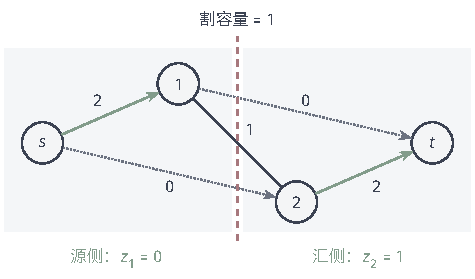
\includegraphics[width=80.405mm]{figures/06-probabilistic-graphical-models/02-inference/tikz/pgm-variational-cut/figure.pdf}
  \caption{两变量次模能量的$s$--$t$割网络。源侧编码为$0$，汇侧编码为$1$；实线终端边容量为$2$，点线终端边容量为$0$，中间无向边容量为$1$。虚线表示分开$\{s,1\}$和$\{2,t\}$的割，容量为$1$，对应配置$(0,1)$。}
  \label{fig:pgm-variational-cut}
\end{figure}

\subsubsection{多标签能量的局部优化}
\label{sec:pgm-variational-multilabel-cuts}

次模图割只解决二值问题。当每个变量有多个标签（不止0/1）时，一次割无法表达全部选择，常用的局部搜索是\emph{反复把多标签问题临时化成二元问题}：$\alpha$扩展每轮挑一个候选标签$\alpha$、让每个节点决定“保留现标签还是改成$\alpha$”（这一步在度量型代价下次模、可精确用图割解），逐轮尝试所有标签直到没有改进；$\alpha$-$\beta$交换则只允许当前标为$\alpha$或$\beta$的节点在这两个标签间重排。它们只保证局部最优，$\alpha$扩展在Potts能量下还有一个“至多两倍最优”的近似比保证。对多标签变量，一次$s$--$t$割只能表达两个选项。\term{$\alpha$扩展}（$\alpha$-expansion）固定当前标签$\ell_i$，让每个节点选择保留$\ell_i$或改为$\alpha$，把这一步化为二元问题。令动作变量$y_i=0$表示保留$\ell_i$、$y_i=1$表示改为$\alpha$，则一条边在四种动作下的代价为
\[
  \begin{array}{ccc}
      &y_j=0&y_j=1\\
    y_i=0&V_{i,j}(\ell_i,\ell_j)&V_{i,j}(\ell_i,\alpha)\\
    y_i=1&V_{i,j}(\alpha,\ell_j)&V_{i,j}(\alpha,\alpha)
  \end{array}.
\]
因此，能够使用上一小节的图割，取决于这张二元表是否次模。若成对项为$w_{i,j}d(k,l)$，$w_{i,j}\geq0$且$d$是标签上的度量，三角不等式给出
\[
  d(\ell_i,\ell_j)+d(\alpha,\alpha)
    \leq d(\ell_i,\alpha)+d(\alpha,\ell_j).
\]
所以每个扩展子问题次模，能精确求解。循环标签并只接受严格改善，有限状态下会停在对所有扩展动作都无法改进的配置，但未必是全局最优。

$\alpha$--$\beta$交换采用另一种二元动作：当前标为$\alpha$或$\beta$的节点是活跃节点，每个活跃节点独立选择$\alpha$或$\beta$，其他节点的标签保持固定。这不是强制两个节点互换标签；活跃节点可以共同改成同一标签。两个活跃节点之间的次模条件为
\[
  V_{i,j}(\alpha,\alpha)+V_{i,j}(\beta,\beta)
    \leq V_{i,j}(\alpha,\beta)+V_{i,j}(\beta,\alpha).
\]
例如，非负、对称且对角值为零的成对代价满足这一条件，即使它不满足标签间的三角不等式。只有一个端点活跃的边，在非活跃端标签固定后成为一元项，因此不会增加二元次模限制。交换由此可处理这类不能直接用于所有扩展动作的代价。

近似比保证还要固定原始能量的形式。对于
\[
  E(\bm\ell)=\sum_iD_i(\ell_i)
       +\sum_{(i,j)\in E}w_{i,j}\mathbb I[\ell_i\ne\ell_j],
  \qquad D_i(k)\geq0,\quad w_{i,j}\geq0,
\]
即非负一元项与非负边权的Potts能量，完全达到扩展局部最优的返回配置$\bm\ell_{\mathrm{return}}$满足经典保证$E(\bm\ell_{\mathrm{return}})\leq2E^\star$，其中$E^\star=\min_{\bm\ell}E(\bm\ell)$。这里要求对每个标签都已没有改善的扩展动作，提前停止并不能直接使用该保证。其他度量或不同停止状态需要相应的近似比分析；能量平移也会改变乘法比值，不能在任意移去常数后仍照用两倍界。更一般的扩展、交换与近似比结果参见Boykov等人\scite{pgm-variational-boykov2001}。

标签本身若有自然次序，还可能利用更强的代价结构。例如，标签为$0,\ldots,K-1$，成对代价为$w_{i,j}g(\ell_i-\ell_j)$、$w_{i,j}\geq0$，且$g$在允许的整数差值上满足$g(r+1)-2g(r)+g(r-1)\geq0$。这个二阶差分条件表示标签差每增加一单位所带来的增量代价不会下降，即离散凸性。在一元代价有限的这一设定下，可以把一个标签编码为一串有序阈值：标签为$k$，就表示它越过前$k$层阈值。多层图用这些阈值节点及保持次序的约束表示标签，在满足相应图表示条件时可一次精确求解。这条路线依赖有序标签和凸代价的结构，不能直接覆盖一般多标签能量\scite{pgm-variational-ishikawa2003}。

一般多标签或非次模能量仍可能需要其他松弛与搜索方法。二元变量的任意成对代价可写成常数、一次项和$z_iz_j$项之和；因为变量取布尔值而函数值取实数，这类目标称为二次伪布尔函数。某些相应松弛，例如具有持久性性质的图割松弛，可返回部分确定的$0/1$标签，其余节点标为未定。这里“确定”的保证是：至少存在一个全局最优配置，与所有已给出的标签相容；它不保证任意补全其余标签都最优。未定部分仍需继续求解、搜索或补全，并在原能量下评价最终配置\scite{pgm-variational-kolmogorov2007qpbo}。

\subsection{可行配置恢复与最优性诊断}

\label{sec:pgm-variational-tightness-rounding}

用松弛/对偶求得可计算上界，再通过取整或图割得到合法配置后，可用原始--对偶间隙评价该配置与最优值的距离。松弛值给出上界，已找到配置的真实得分给出下界；二者之差构成无需知道真值的次优性证书，间隙为零即证明全局最优。分数解在次模或树结构下可以无损取整，此时松弛是紧的。对于二元次模能量，共同阈值取整可以直接证明局部LP松弛是紧的。令$m_i=\mu_i(1)$。对任何局部一致的边表，$\Pr(Z_i\ne Z_j)\geq|m_i-m_j|$，因为$m_i-m_j=\mu_{i,j}(1,0)-\mu_{i,j}(0,1)$。非负$w_{i,j}$使松弛能量不小于
\[
  C+\sum_i[(1-m_i)D'_i(0)+m_iD'_i(1)]
       +\sum_{(i,j)}w_{i,j}|m_i-m_j|.
\]

令所有节点共用$U\sim\operatorname{Uniform}(0,1)$，取$z_i=\mathbb I[U<m_i]$，则节点均值为$m_i$，不同值概率恰为$|m_i-m_j|$。这个全局分布的期望能量等于上式，所以至少有一个阈值配置的能量不高于原LP解。用于LP最优解时，结合松弛下界便得到整数最优值等于LP最优值。因此LP存在整数最优解；存在平局时，若干整数最优解的分数混合也可能达到同一最优值。按排序后的$m_i$检查至多$d+1$个阈值区间即可寻找相应配置。

树图上的局部LP同样是紧的。局部一致表可以构造全局树分布，其期望得分不超过某个配置的得分，因此松弛最优值等于整数最优值，并存在整数最优解。树上的一般边缘仍可以是分数。含环图的紧性需要结合结构、势函数与参数判断，消息收敛本身只说明更新的状态。

对于一般LP分数解，可以逐点选择最大伪边缘、联合取整、局部搜索，或使用切平面和分支定界。逐点选择可能破坏变量之间的协调；存在硬约束时，还需检查恢复的配置是否可行，并在原目标下计算其得分。

对得分最大化，保留已找到的最好可行值$L=S(\widehat{\bm z})$及一个经验证的对偶上界$U$，则
\begin{equation}
  0\leq M-S(\widehat{\bm z})\leq U-S(\widehat{\bm z}).
  \label{eq:pgm-variational-gap}
\end{equation}
右侧是可计算的\term{原始--对偶间隙}（primal--dual gap），在此处比较整数可行解与松弛对偶证书。若还记录一个LP原始可行解$\bm\mu$的目标值$P=\langle\bm\theta,\bm\mu\rangle$，就能增加对求解过程的诊断，但要区分几个不同对象。对同一个LP及其对偶，有
\[
  U\geq U_{\mathrm{LP}}\geq M\geq L,
  \qquad P\leq U_{\mathrm{LP}}.
\]
其中$U$是对偶可行值，$U_{\mathrm{LP}}$是LP真正的最优值；$P$只是在当前分数可行点达到的值。由第一条链可知，$U-L$确实控制当前整数配置的次优损失。由第二条关系可知，$U-P\geq0$是可计算的LP求解差距，并且同时满足$0\leq U-U_{\mathrm{LP}}\leq U-P$与$0\leq U_{\mathrm{LP}}-P\leq U-P$。所以$U-P$小时，LP原始、对偶两侧的目标值都已接近LP最优值。

$P$与$L$之间却没有固定的大小关系。尚未充分优化的分数点可能比已经找到的合法配置得分还低，因此$P-L$不能无条件称为非负的“取整损失”。即使已经知道$P=U_{\mathrm{LP}}$，$P-L$也同时包含LP与整数问题的差别以及当前配置尚未最优的差别。更完整的关系为
\[
  U-L
    =(U-U_{\mathrm{LP}})
       +(U_{\mathrm{LP}}-M)+(M-L).
\]
三项依次是对偶尚未优化到LP最优值的差距、LP松弛间隙、当前配置相对整数最优值的次优损失，均非负。通常$U_{\mathrm{LP}}$和$M$并未知晓，后两项尤其不能仅凭当前$U,P,L$分别观测；记录三个当前值能提供证据，却不能自动完成这一分解。

对能量最小化，方向反过来：松弛或对偶提供下界，可行配置提供上界。在三角例中，逐点按平局选$0$得到得分$0$；把任一变量翻转便达到$2\beta$，但LP上界仍为$3\beta$。由于本例的整数真值与LP最优值都能独立算出，可以明确判断局部改进消除了当前配置的次优损失，却没有修复$\beta$的松弛间隙。再取三角例的均匀独立分布所诱导的局部表，得到LP原始可行值$P=3\beta/2$；与刚才的合法配置$L=2\beta$相比，$P-L=-\beta/2<0$，直接显示两者不具有固定顺序。

LP对偶的凸性支持全局求解，但求得$U_{\mathrm{LP}}$后，整数最优值仍可能更低。若一个合法配置达到对偶值，则配置与上界之间的间隙为零，可以立即形成全局最优证书。对于TRW消息算法，还需检查具体调度如何优化上界；目标的凸性与某种更新的单调性属于不同的论证。

MPE分解把计算分配给子问题。成对树上的一次最大和及回溯需$O(|E_T|k^2)$；多棵树可并行，但共享乘子的协调和通信仍在。显式局部LP有约$O(dk+mk^2)$个变量，其求解时间不只由变量数决定，还受求解器、约束和容差影响。图割属于多项式时间的特殊精确子问题，一次扩展只解一个二元动作，整体还要计入标签轮数。衡量可扩展性时，应同时报告单轮计算、存储、通信和达到所需诊断标准的轮数。

MPE近似需要另一套记录：原约束是否满足、可行配置得分是多少、对偶上界是多少，以及它们的差距。三角图的结论可同时列出：完全平均场的对数配分函数下界为$3.119162$，结构化固定点的同类下界为$3.178054$，精确$\log Z_\beta=3.258097$，Bethe固定点的对数配分函数近似为$3.295837$。MPE方面，最好可行得分为$2\log2=1.386294$，LP与该树分解的上界为$3\log2=2.079442$。前一组数值比较对数配分函数，后一组比较最大配置得分；它们需要分别展示对应的真值与界。

原始--对偶间隙直接控制当前配置相对于最优得分的损失。后验是否集中在该配置附近，以及各变量的边缘概率，还需由分布查询回答。间隙较大时，先用可计算的$U-P$检查LP是否还未求解充分，再尝试改进合法配置或加强一致性约束。对偶优化误差、松弛间隙和配置次优损失是不同来源；除非另有精确解或证书，不能声称已经把它们分别测出。可以根据现有上下界及改进结果，选择继续求解、加强松弛或接受已量化的总误差范围。配置推断的结果应同时包含合法配置及其得分证书。

\section{本章小结}

\label{sec:pgm-variational-summary}

本章以已知模型下的两类查询组织近似推断。对于后验分布，ELBO用反向KL连接近似分布与目标；平均场和结构化VI通过限制$q$的依赖，使期望和真实熵可计算。共轭消息、小批量更新与摊销映射分别减少局部期望计算、数据遍历和逐样本优化的成本，近似族误差则取决于所保留的结构。

局部自由能维护伪边缘，以局部一致性和熵近似替代全局分布计算。树上这些关系精确，推广到含环图后形成Bethe与Kikuchi近似；更大的区域保留更多联合约束，也增加表格和通信成本。EP以倾斜分布的矩修正站点，拉普拉斯法用峰附近曲率构造高斯。各方法的优化或固定点性质需要与实际概率查询的误差分别检查。

对于全部非证据变量的MPE，目标是最大配置得分。边缘多面体上的线性优化与这一查询等价，局部多面体松弛给出上界，对偶分解与TRW便于计算证书，二元次模等特殊结构可用图割直接返回整数最优解。配置结果通过可行性和原始--对偶间隙诊断，分布结果通过支持、相关性和预测诊断。含求和变量的边缘MAP还需保留其求和运算，另按对应查询求解。

\paragraph{扩展阅读}
Wainwright与Jordan系统联系了指数族、变分目标和图结构，可用于进一步理解边缘多面体与熵对偶。阅读时可围绕近似边缘、最优配置和配分函数分别比较目标、可行域及界的方向，并考察局部计算所保留的依赖\scite{pgm-wainwright2008}。
